%\documentclass[<options>]{elsarticle}
\documentclass [sort&compress] {elsarticle}
\usepackage{graphicx}% Include figure files

\bibliographystyle{elsarticle-num}
\begin{document}
\begin{frontmatter}

\title{Relationship between the ideality factor and the iron concentration in silicon solar cells}

\author{O.Ya.~Olikh}
\ead{olikh@univ.kiev.ua}

\address{Faculty of Physics, Taras Shevchenko National University of Kyiv, Kyiv 01601, Ukraine}


\begin{abstract}

In this work numerical simulator SCAPS (Solar Cell Capacitance Simulator) is used to elucidate this phenomenon.

The influence of ultrasound on current--voltage characteristics of crystalline silicon solar sell was investigated experimentally.
The transverse and longitudinal acoustic waves were used over a temperature range of 290--340~K.
It was found that the ultrasound loading leads to the reversible decrease in the photogenerated current, open--circuit voltage, fill factor, carrier lifetime, and shunt resistance as well as the increase in the ideality factor.
The experimental results were described by using the models of coupled defect level recombination, Shockley--Read--Hall recombination, and dislocation--induced impedance.
The contribution of the boron-�oxygen related defects, iron-�boron pairs, and oxide precipitates to both the carrier recombination and acousto--defect interaction was discussed.
The experimentally observed phenomena are associated with the increase in the distance between coupled defects as well as the extension of the carrier capture coefficient of complex point defects and dislocations.
\end{abstract}

%\pacs{73.30.+y, 43.35.Ty, 43.35.+d, 72.20.-i, 73.40.-c}

\begin{keyword}
silicon solar cell\sep simulation\sep ideality factor\sep iron concentration
\end{keyword}

\end{frontmatter}


\section{Introduction}

It is well known that impurities are crucial for the semiconductor devices performance.
It is completely relevant to solar cell (SC) as well.
Dopants determinate an internal electric field, which leads to a separation of light-generated carriers and a photovoltage generation.
Contaminants act often as a highly effective recombination centre, reducing the carrier lifetime and SC efficiency.
Therefore the impurity concentration determination is a very important problem.
There are many experimental methods for solving this problem, such as the infrared spectroscopy, deep level transient spectroscopy, photoluminescence,
thermally stimulated capacitance and current, secondary ion mass spectrometry etc \cite{Schroder2006}.
These methods are complicated  enough and demand a special setup.

At the same time, the analysis of  the current--voltage ($I-V$)  characteristic is commonly used  to characterize the solar cell.
Thus, the dark $I-V$ curve normally serves as a first diagnosis of SC recombination \cite{Grover}.
The $I-V$  equation that models the SC by an equivalent electrical circuit contains several parameters related to physical phenomena occurring in the device.
It is obviously that these parameters depend on impurities, but the interrelations are intricate sufficiently.
As a result, $I-V$ curves are not used practically for a contaminant diagnosis, although the possibility of simultaneous calibrate both SC performance and impurity looks quite attractive.

One of a number of parameters of SC model is ideality factor $n$.
If the defect related recombination  is a prevailing process within  a  space charge region than the value $n=2$ is often stated in a literature.
But it  is  only  the  very specific  assumptions about  the  energy levels  (middle  of  the  bandgap) and  capture  cross sections  (equal for electrons and  holes)  of  the
recombination centres in a symmetrically  doped diode which lead to $n=2$ \cite{n2Kuhn,n2_Beier}.
A discrepancy between this $n=2$--theory and experiment is observed and a $n$ value depends on SC ambient conditions and the parameters of the recombination centers, particularly  their concentration \cite{n2_Beier,n2McIntosh,n2Kaminski,HAMEIRI2013251,Heide}.

The aim of our work is to investigate a possibility of  a contaminant concentration evaluation by using an ideality factor value.
The heuristic approach is used and its milestones can be expressed as following:
i)~the dark $I-V$ characteristic of the SCs with known contaminant composition is simulated;
ii)~the obtained characteristic is fitted according to the double--diode model and the ideality factor is determined;
iii)~the initial impurity concentration and the calculated ideality factor value are used for acquisition of analytic or grading dependencies.

As a first step, the paper considers a fairly simple but practically important system.
Namely, the crystalline silicon SC and iron impurity were under consideration.
Si photovoltaic device cover almost 90\% of global SC market.
Iron is a major contaminant due to the wide use of stainless steel equipment in the fabrication line and one of the most detrimental metal impurities in solar--grade crystalline silicon materials \cite{Istratov1999,FeB:Schmidt,ZHU2016192}.

Numerical simulation is carried out using the one--dimensional code SCAPS \cite{SCAPS1,SCAPS2}.
This software is widely used to modeling of various solar cells \cite{SCAPSuse1,SCAPSuse2,SCAPSuse3,SCAPSuse4,SCAPSuseSi1,SCAPSuseSi2,SCAPSuseSi3},
including silicon based devices \cite{SCAPSuseSi1,SCAPSuseSi2,SCAPSuseSi3}.

\section{Simulation details}
\subsection{Solar cell structure and material parameters}
The simple structure, which is used in the SC simulations, is  shown on inset in Fig.~\ref{figIV}.
The main used parameters are listed in Table~\ref{tabSC}.


\begin{table}
\caption{\label{tabSC}Parameters of the simulated solar cell.
}
\begin{tabular}{lcl}
\hline
\hline
Parameter&Symbol&Value\\
\hline
Emitter thickness & $d_n$ &0.5~$~\mu$m\\
Base thickness & $d_p$ &300~$~\mu$m\\
Emitter Doping (n--type, uniform)& $N_\mathrm{D}$ &$10^{19}$~cm$^{-3}$\\
Base Doping (p-type, uniform)& $N_\mathrm{A}$ &$10^{15}\div 10^{17}$~cm$^{-3}$\\
Iron content (base, uniform) & $N_{\mathrm{Fe}}$ &$10^{10}\div 10^{13}$~cm$^{-3}$\\
Temperature & $T$ &$290\div330$~K\\
%8.0&longitudinal&0.18&1.3&0.3&lUL&SC4, SC15\\
%4.2&transverse&0.19&2.8&0.6&tULa&SC15\\
%4.2&transverse&0.22&3.1&0.7&tULb&SC4\\
%4.2&transverse&0.40&4.2&0.9&tULc&SC4, SC15\\
\hline
\hline
\end{tabular}
\end{table}

In our simulation, the temperature dependencies of bandgap and carrier mobility are calculated, respectively,  according to Varshni and Caughey--Thomas equations \cite{Schroder2006}.
Bandgap narrowing is considered as described by the Slotboom equation \cite{Markvart,ZHOU20188}.
The density of states in the conduction/valence band ($N_C$/$N_V$) and thermal carrier velocities are from Green \cite{Nc:Green}.

%It should be noted that the SCAPS takes into account the simplified temperature dependencies of density of states in the conduction/valence band
%($N_C$/$N_V$) and  thermal electron/hole velocity ($\upsilon_{\mathrm{th},n}$/$\upsilon_{\mathrm{th},p}$) only.

The iron atoms are known to be located in interstitial lattice position in silicon, predominantly.
The donor level $E_{\mathrm{Fe}_i} = E_V+0.394$~eV is associated with $\mathrm{Fe}_i$ \cite{Rein2,MurphyJAP2011}.
Therefore neutral  interstitial  iron  $\mathrm{Fe}_i^0$ and interstitial ionized iron $\mathrm{Fe}_i^+$   are observed in  Si.
In $p$--type material, $\mathrm{Fe}_i^+$ readily interacts with ionized shallow acceptors.
In our simulation, the boron is a dopant impurity and the pair $\mathrm{Fe}_i\mathrm{B}_s$ must be under consideration.
On the one hand, this pair is bistable defect and the trigonal and the orthorhombic configuration are feasible.
On the other hand, the orthorhombic pair is only observable at low temperature ($<150$~K) under an illumination or carrier injection condition \cite{Narland,Sakauchi}.
Besides  the $\mathrm{Fe}_i\mathrm{B}_s$ pairs can be readily dissociated by 15 to 90~s illumination with a halogen lamp \cite{FeB:Schmidt}.
The association reaction is diffusion limited and can take place under dark condition during tens minute \cite{FeB:kinetic}.
Two following cases are under simulation.


\noindent
i)~
%All iron atoms are isolated interstitial:
We assume a negligible proportion of Fe present in the form of FeB pairs:
\begin{equation}
\label{eqN1}
    N_{\mathrm{Fe}}=N_{\mathrm{Fe}_i^0}+N_{\mathrm{Fe}_i^+} \,,
\end{equation}
where
$N_{\mathrm{Fe}_i^0}$ and $N_{\mathrm{Fe}_i^+}$ are the concentrations of  neutral and ionized iron respectively.
This is a safe assumption for cells operating under constant illumination or after illumination stop immediately.
%ProgPVResAppl_8_p363.pdf
%Such condition is realisable  after illumination immediately.
The interstitial iron is considered as uniform in the SC base,
the hole and electron capture cross--sections of defect are calculated according to
$\sigma_{p,\mathrm{Fe}_i}=3.85\times10^{-16}\exp(-0.045/kT)$~cm$^2$ and
$\sigma_{n,\mathrm{Fe}_i}=9.1\times10^{-15}\exp(-0.024/kT)$~cm$^2$ \cite{Istratov1999,Rein2,MurphyJAP2011}.
$E_{\mathrm{Fe}_i}$ is taken as the temperature independent value \cite{Kohno}.
This case is labeled ``FI'' from now on.

\noindent
ii)~The total dissolved iron concentration is given by a sum of concentrations of three separate species, $\mathrm{Fe}_i^0$, $\mathrm{Fe}_i^+$,
and iron paired with an boron:
\begin{equation}
\label{eqN2}
    N_{\mathrm{Fe}}=N_{\mathrm{Fe}_i^0}+N_{\mathrm{Fe}_i^+}+N_{\mathrm{FeB}}=N_{\mathrm{Fe}_i}+N_\mathrm{FeB} \,,
\end{equation}
where
$N_\mathrm{FeB}$ is the pair concentration,
$N_{\mathrm{Fe}_i}$ is the concentration of unpaired interstitial iron.
This case corresponds to an equilibrium condition.
The equilibrium concentration of $\mathrm{Fe}_i^+$  is given by \cite{MurphyJAP2011,FeB:kinetic}
\begin{equation}
\label{eqNFe+}
    N_{\mathrm{Fe}_i^+}=\frac{N_{\mathrm{Fe}}}{\left[1+N_\mathrm{A}10^{-23}\exp\left(-\frac{E_b}{kT}\right)\right]\left[1+\exp\left(-\frac{F-E_{\mathrm{Fe}_i}}{kT}\right)\right]}\,,
\end{equation}
where
$F$ is the Fermi level,
$E_b$ is the binding energy of the FeB pairs (taken as 0.582 eV).
Since the $\mathrm{Fe}_i^0$  species are  in local  equilibrium with both  isolated $\mathrm{Fe}_i^+$  atoms  and
$\mathrm{Fe}_i^+$ atoms which  are  associated in the FeB--pairs, the following expression silicon may be written as \cite{FeB:kinetic}
\begin{equation}
\label{eqNrel}
    \frac{N_{\mathrm{FeB}}+N_{\mathrm{Fe}_i^+}}{N_{\mathrm{Fe}_i^0}}=\exp\left(-\frac{F-E_{\mathrm{Fe}_i}}{kT}\right) \,.
\end{equation}
A simple transformation of Eqs.~(\ref{eqN2})--(\ref{eqNrel}) enables one to obtain the following expression for relationship between total iron concentration and pair concentration
\begin{equation}
\label{eqNFeB}
    N_{\mathrm{FeB}}=N_{\mathrm{Fe}}\frac{N_\mathrm{A}10^{-23}\exp\left(-\frac{E_b}{kT}\right)}
     {\left[1+N_\mathrm{A}10^{-23}\exp\left(-\frac{E_b}{kT}\right)\right]\left[1+\exp\left(-\frac{F-E_{\mathrm{Fe}_i}}{kT}\right)\right]}\,.
\end{equation}
The Fermi level position is not uniform in the SC base.
Hence FeB pair concentration is not uniform as well even if iron content is uniform.

In our simulation, the Fermi level position in the SC base Has been calculated for each doping and temperature values.
Then Eq.~\ref{eqNFeB} was used to calculate the FeB pair distribution.
The representative example of calculation is shown in Fig.~\ref{figDist}.

\begin{figure}
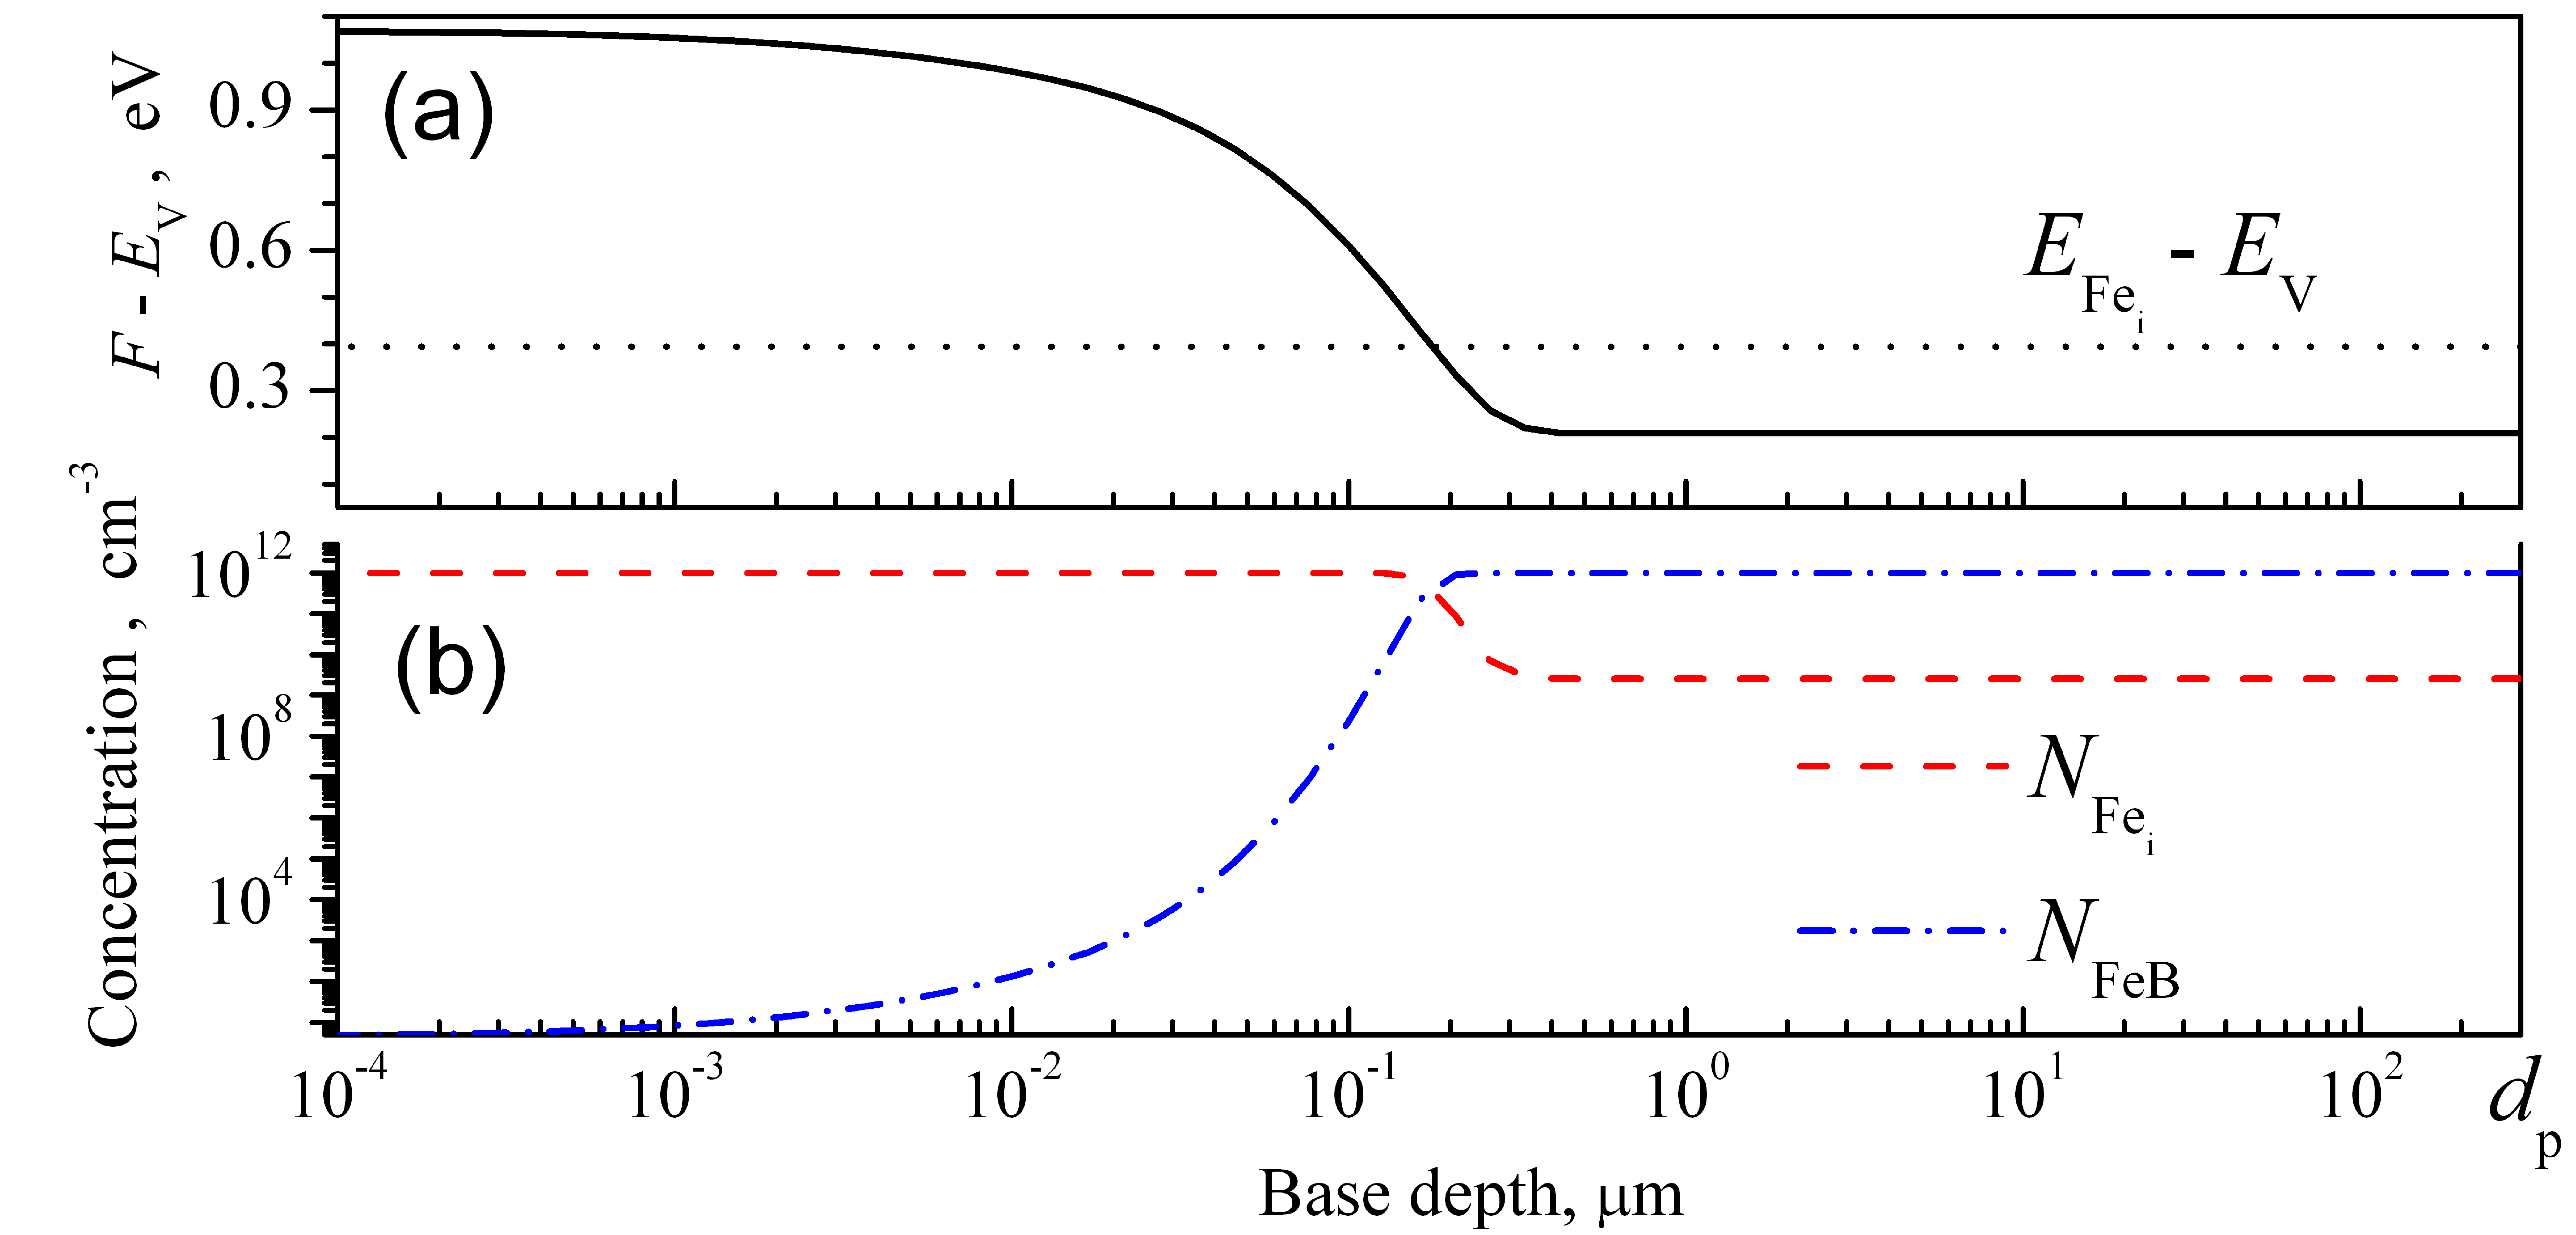
\includegraphics[width=12cm]{Fig2}%
\caption{\label{figDist}
The calculated SC base distribution of Fermi level position (a, solid line), unpaired interstitial iron concentration (b, dashed line),
and FeB pair concentration (b, dotted--dashed line).
$N_\mathrm{A}=10^{16}$~cm$^{-3}$, $T=300$~K.
The position of $\mathrm{Fe}_i$ donor level (dotted line) is shown in the panel (a) as well.
}%
\end{figure}


%In the following analysis, Teff is considered approximately equal to 1, a true condition for quasi-ballistic devices.

The trigonal FeB pair is considered, a true condition under room temperature.
This pair is amphoteric defect.
In the following analysis, the parameters of donor ($E_{\mathrm{FeB}}^{d} = E_V+0.10$~eV,
$\sigma_{p,\mathrm{FeB}}^d=2\times10^{-14}$~cm$^2$,
$\sigma_{n,\mathrm{FeB}}^d=4\times10^{-13}$~cm$^2$)
and  acceptor ($E_{\mathrm{FeB}}^{a} = E_C-0.26$~eV,
$\sigma_{p,\mathrm{FeB}}^a=5.5\times10^{-15}$~cm$^2$,
$\sigma_{n,\mathrm{FeB}}^a=2.5\times10^{-15}$~cm$^2$)
levels are used from \cite{Istratov1999,Rein2,MurphyJAP2011,FeB:kinetic}.
This case is labeled ``FIFB'' from now on.

Only a bulk recombination is under consideration in the paper.
Once again two cases are simulated.
In the first one, labeled ``SRH'', the Shockley--Read--Hall recombination is taken into account only.
In the second one, denoted ``SRHBBA'', the both Shockley--Read--Hall recombination and intrinsic recombination are allowed for.
The electron and hole Auger recombination factors ($C_n=2.8\times10^{-31}$~cm$^6$s$^{-1}$ and $C_p=9.9\times10^{-32}$~cm$^6$s$^{-1}$) 
and radiative band--to--band recombination coefficient ($B=1.8\times10^{-15}$~cm$^3$s$^{-1}$) 
are taken from \cite{Markvart}.

So, four different data sets (FI--SRH, FI--SRHBBA, FIFB--SRH, and FIFB--SRHBBA)
have been simulated for solar cell.


\begin{figure}
%\begin{center}
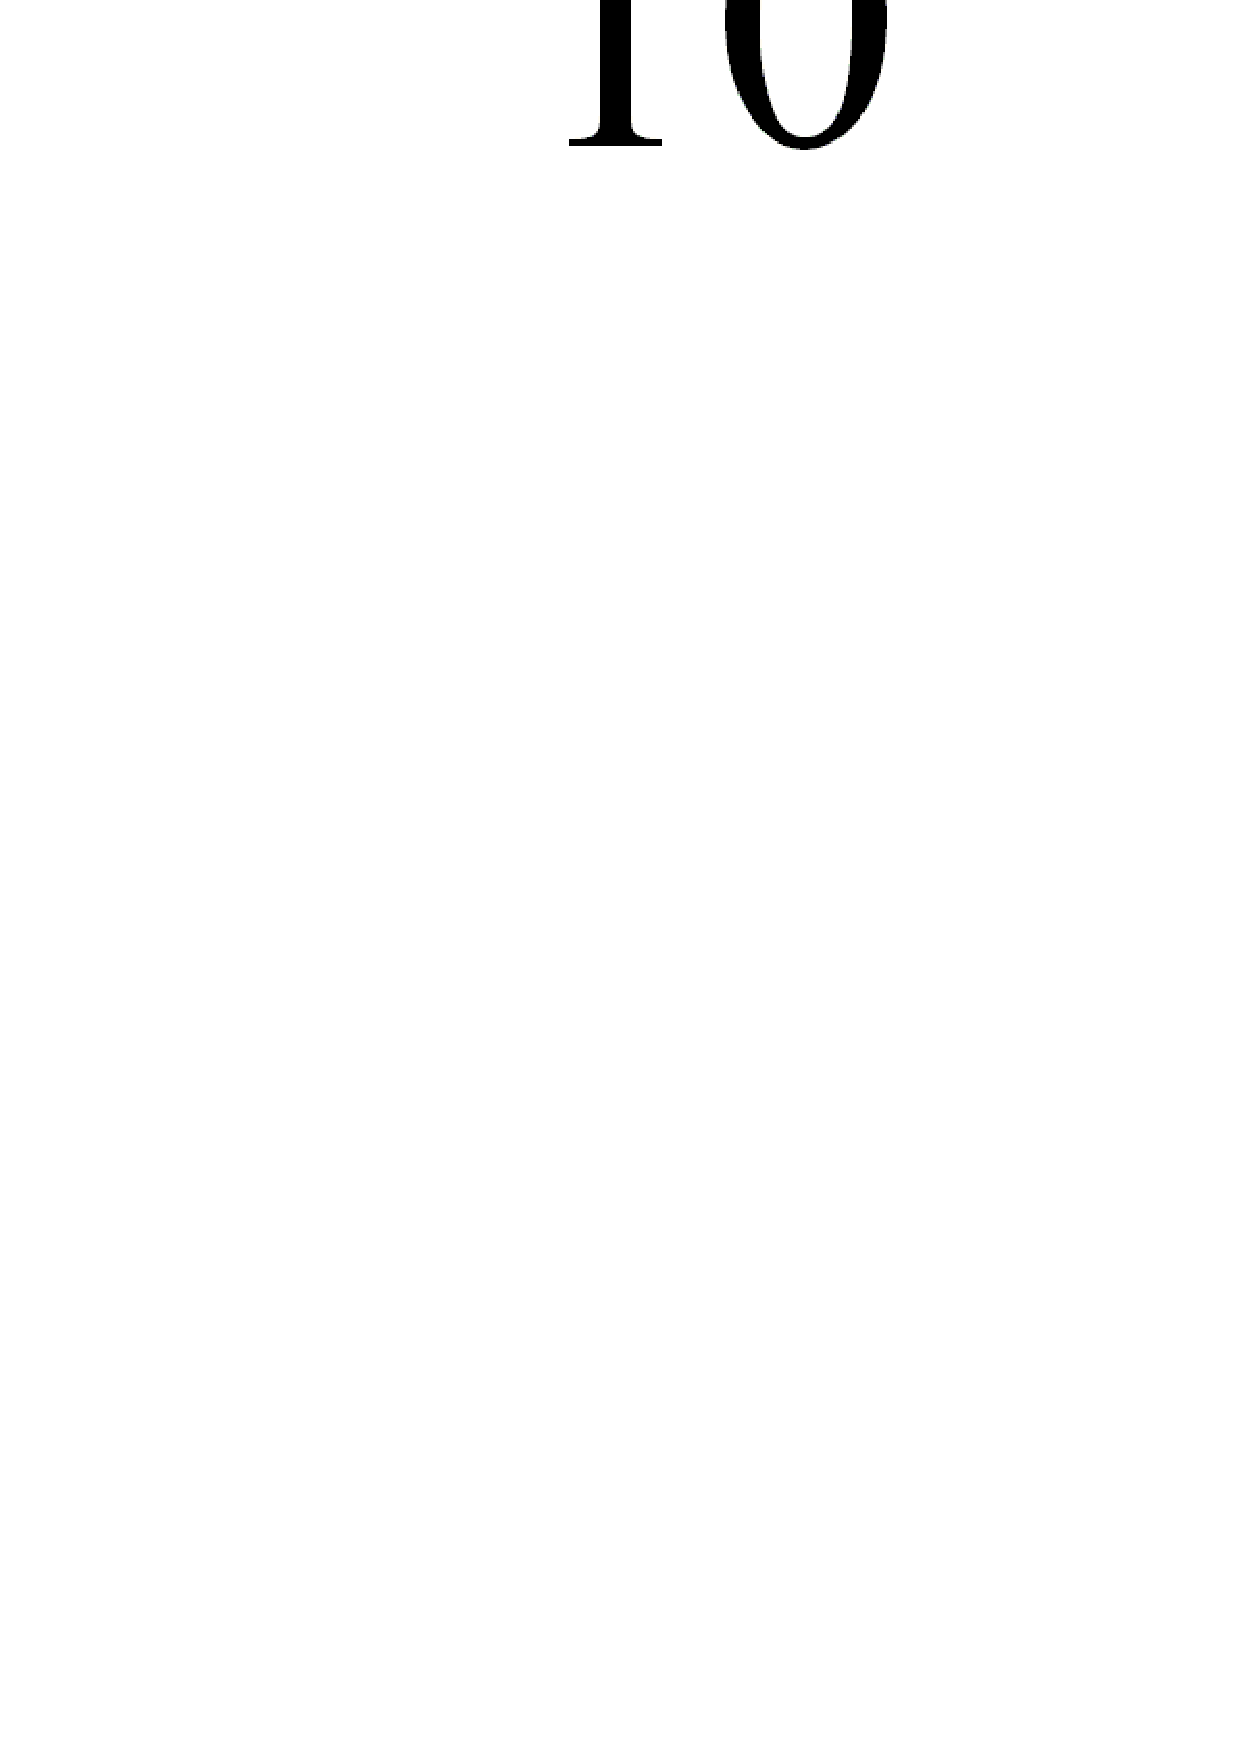
\includegraphics[width=1.0\textwidth]{Fig1}%
%\end{center}
\caption{\label{figIV}
$I-V$ characteristic simulated in FI--SRH--case, $N_\mathrm{A}=10^{17}$~cm$^{-3}$,  $N_{\mathrm{Fe}}=10^{13}$~cm$^{-3}$, $T=290$~K (marks)
and its fitting by Eq.~(\ref{eqIV}) (solid line).
The dashed and dotted--dashed lines represent the diffusion and recombination currents.
Inset: Solar cell structure, which are used in simulation.
}%
\end{figure}

The dark forward $I-V$ characteristic were generated by SCAPS over a voltage range up to $0.62$~V.
The $I-V$ curve example is shown in Fig.~\ref{figIV}.

The real silicon SCs are often described by so--called two--diode model \cite{Breitenstein2013}.
The first diode represents the ``ideal'' diode, describing the so--called diffusion current, characterized by a saturation current $I_{01}$,
and the second diode is the so--called recombination current, characterized by a saturation current $I_{02}$ and an ideality factor $n$ \cite{Breitenstein2013}.
According to the two--diode model, the dark SC current is given by
\begin{equation}
\label{eqIV}
    I=I_{01}\left[\exp\left(-\frac{qV}{kT}\right)-1\right]+ I_{02}\left[\exp\left(-\frac{qV}{nkT}\right)-1\right]\,.
\end{equation}
It should be noted that the influence of series resistance as well as shunt resistance is neglected in Eq.~\ref{eqIV}.
We used Eq.~\ref{eqIV} to fit the simulated data taking $n$, $I_{01}$, and $I_{02}$ as the fitting parameters and more attention was paid to the ideality factor value.
The fitting result is shown in Fig.~\ref{figIV}.

All non-linear fittings in the paper were done by using the differential evolution method \cite{DE:Sun,DEWang}.
The least--squares method was used to linear fitting.



%We have used two approaches to calculate the depletion region. The first approach is based
%
%In the following analysis, Teff is considered approximately equal to 1, a true condition for quasi-ballistic devices.
%
%Fig. 5 displays themeasured TCs of the FF of the studied cells and that of record silicon cells together with a generic theoretical calculation (green line) and speci?c theoretical predictions based on experimental values for each cell (triangles).
%
%In our simulation, themodel for dopant ionization is from Altermatt et al. [18]. The intrinsic carrier concentration is calculated according to models from Couderc et al. [19]. The bandgap and bandgap narrowing models are, respectively, from Passler [20] and Yan and Cuevas [21]. The thermal velocity is calculated from models by Green [22]. (IEEEJPhotovol_7_p1092-1097.pdf)
%
%
%FeB pairs can be reversibly dissociated either by a thermal anneal of the samples at 200 C for 10min followed by a quench, or by 15 to 90 s illumination with a halogen lamp.
%PR_Istratov_obzor2_ApplPhysA_70_p489_534.pdf
%
%In this work, the electrical parameters of a silicon solar cell are investigated theoretically using a one dimensional model
%
%The intrinsic recombination can be subdivided into radiative and Auger recombination
%
%20. Bandgap narrowing is considered as described by the Slotboom equation [24]:
%(MatSciSemProc_86_p8.pdf,  D:\Literat\Stat\IVchar\PN\Manufacturing\)

%Applying this model, a virtual population of 500 I�V
%curves whose two-diode parameters (JL, J01, J02, Rs, Rp)
%are randomly chosen into representative ranges for crystal-
%line silicon-based solar cells is generated (see [15] and the
%references therein).




\section{Results and Discussion}
\subsection{Interstitial iron, SRH recombination}

Some data, calculated in the FI--SRH case, are shown in Fig.~\ref{figA}(a,b).
One can see that the ideality factor  increases monotonically with the doping level increase.
While temperature dependence of the  $n$  is more intricate: it contains the both increasing and decreasing components and the contribution of the last one rises with  increase in $N_\mathrm{A}$.
The iron concentration increase leads to  the increase in $n$ value and does not change $n(N_\mathrm{A},T)$ dependence --- see Fig.~\ref{figA} and Supplementary Materials.
It is evidence of for possibilities of  $N_\mathrm{Fe}$ evaluation by using $n$.
Only low doping level value ($N_\mathrm{A}\cong10^{15}$~cm$^{-3}$)and high temperature ($T>300$~K) are exclusion 
because $n\cong1$ is expected accordingly to the simulation.

\begin{figure}
%\begin{center}
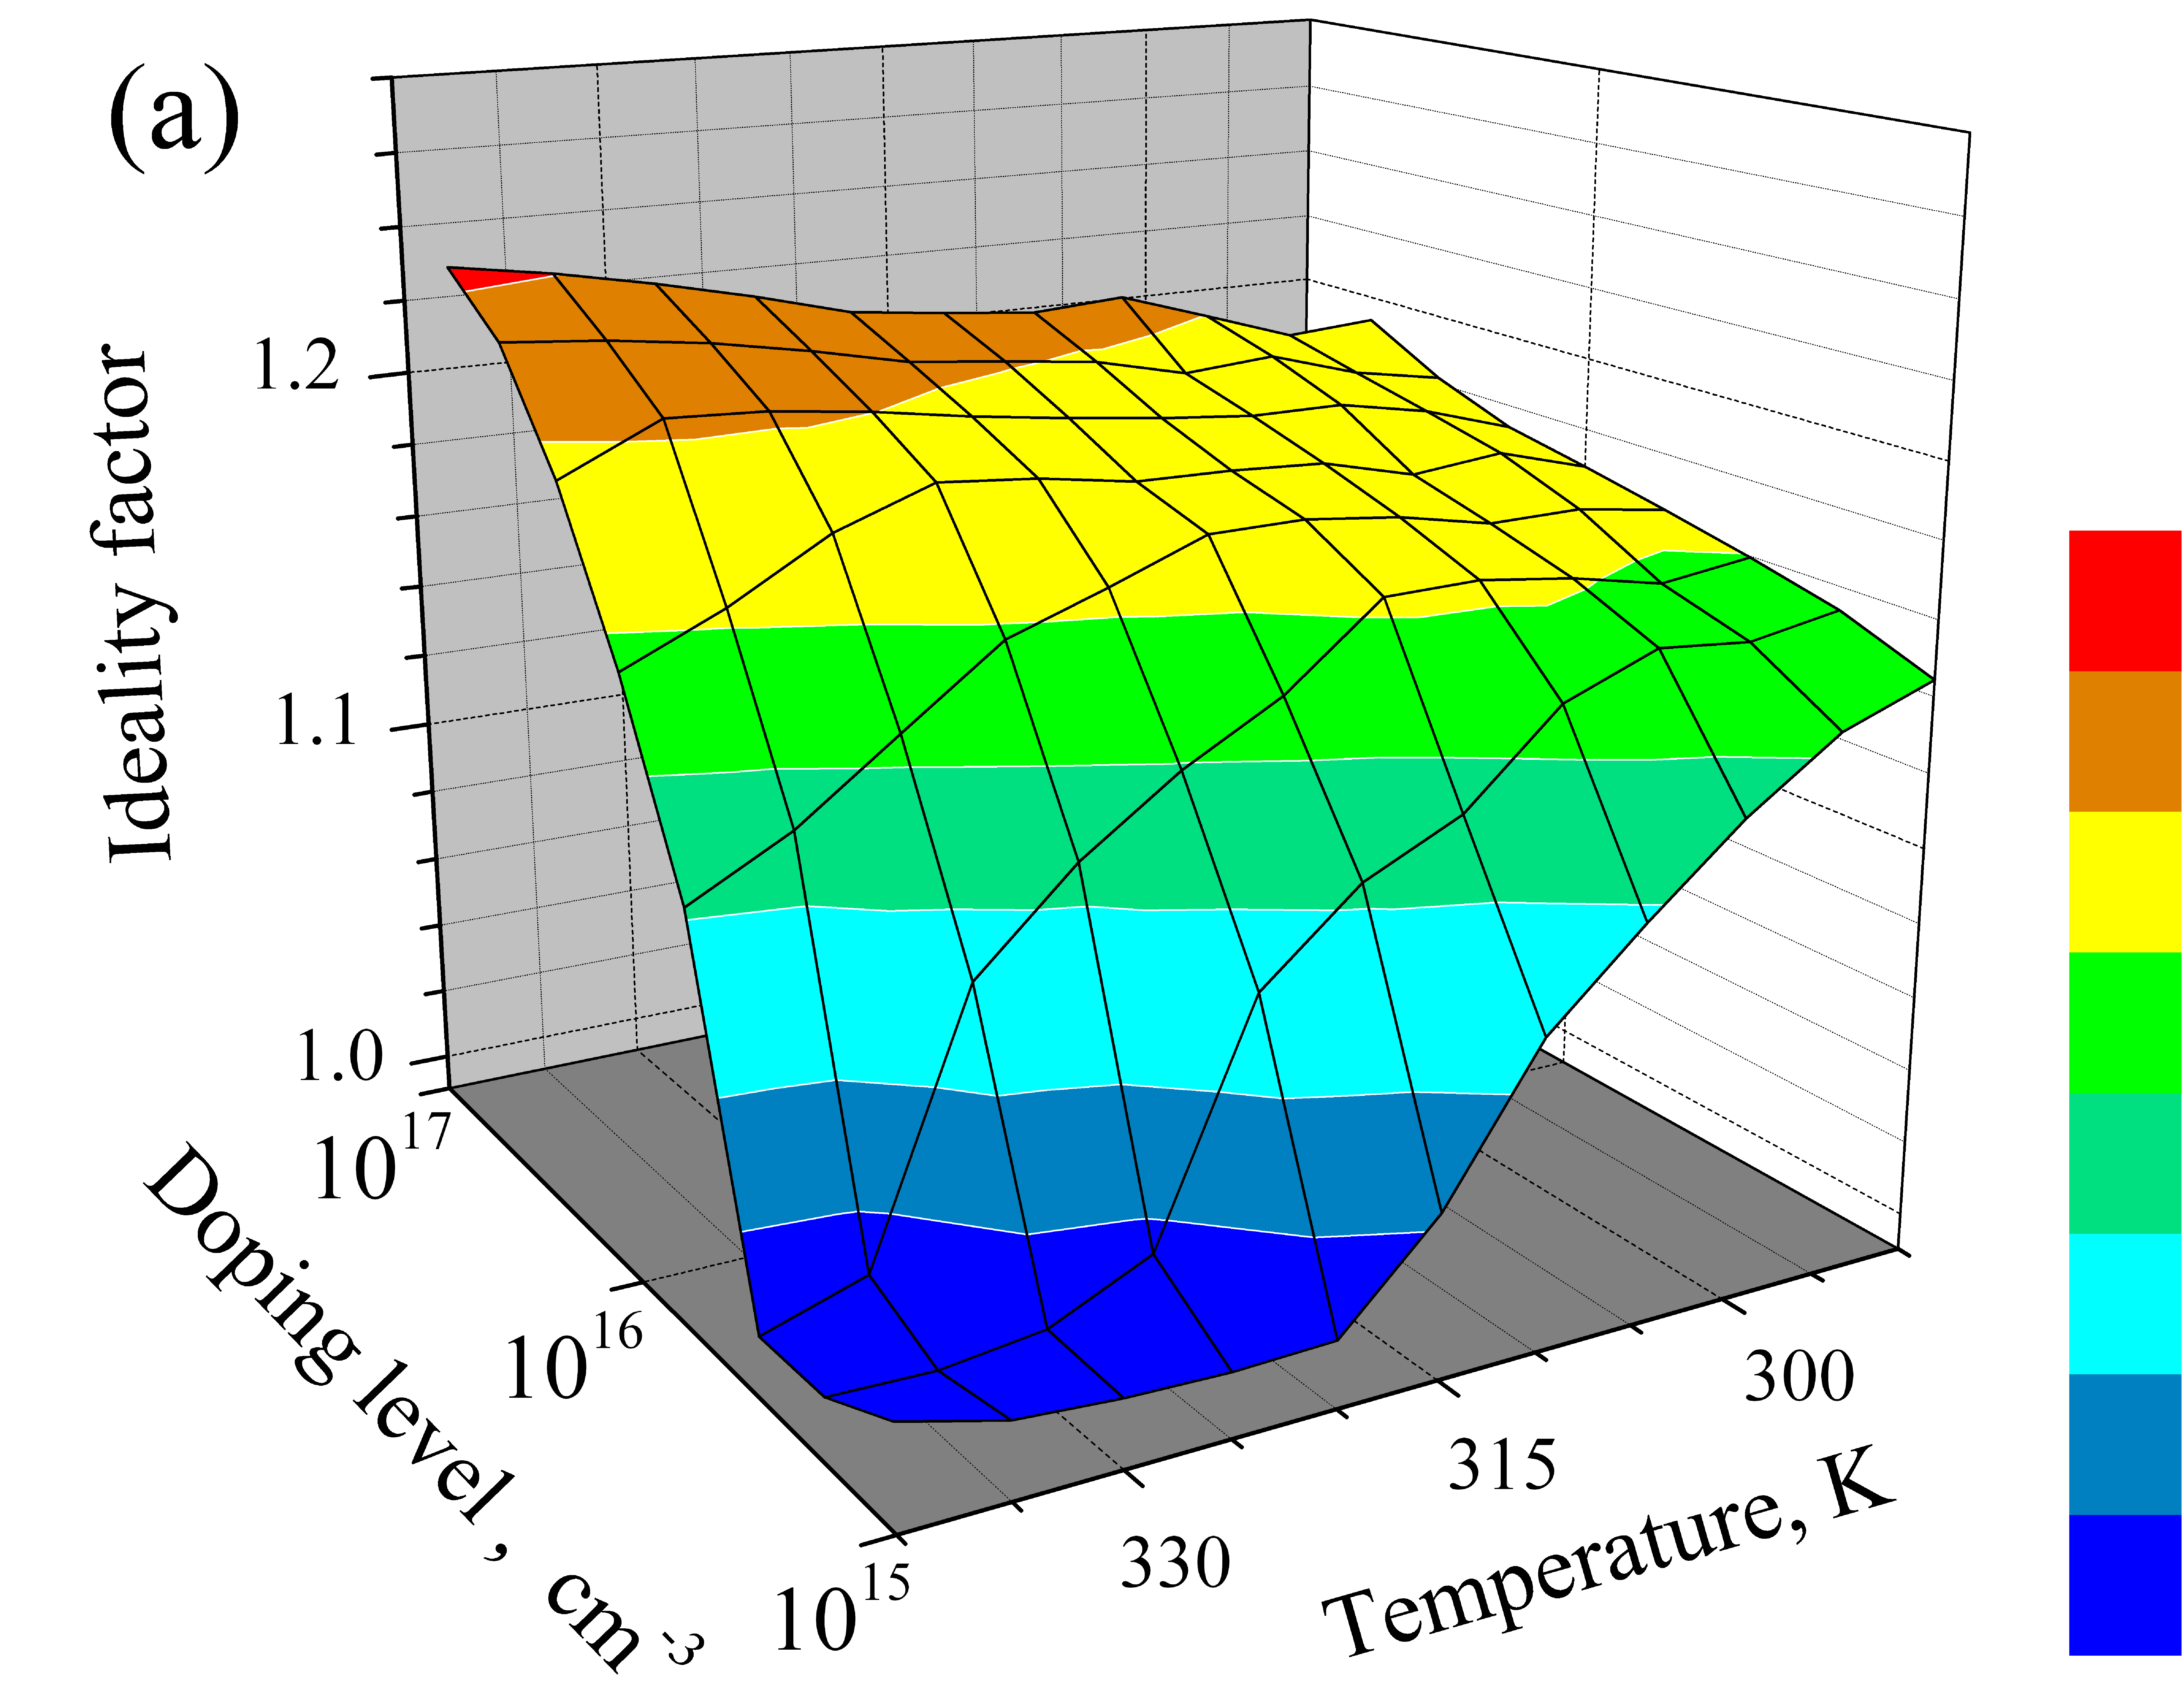
\includegraphics[width=0.5\textwidth]{Fig3a}%
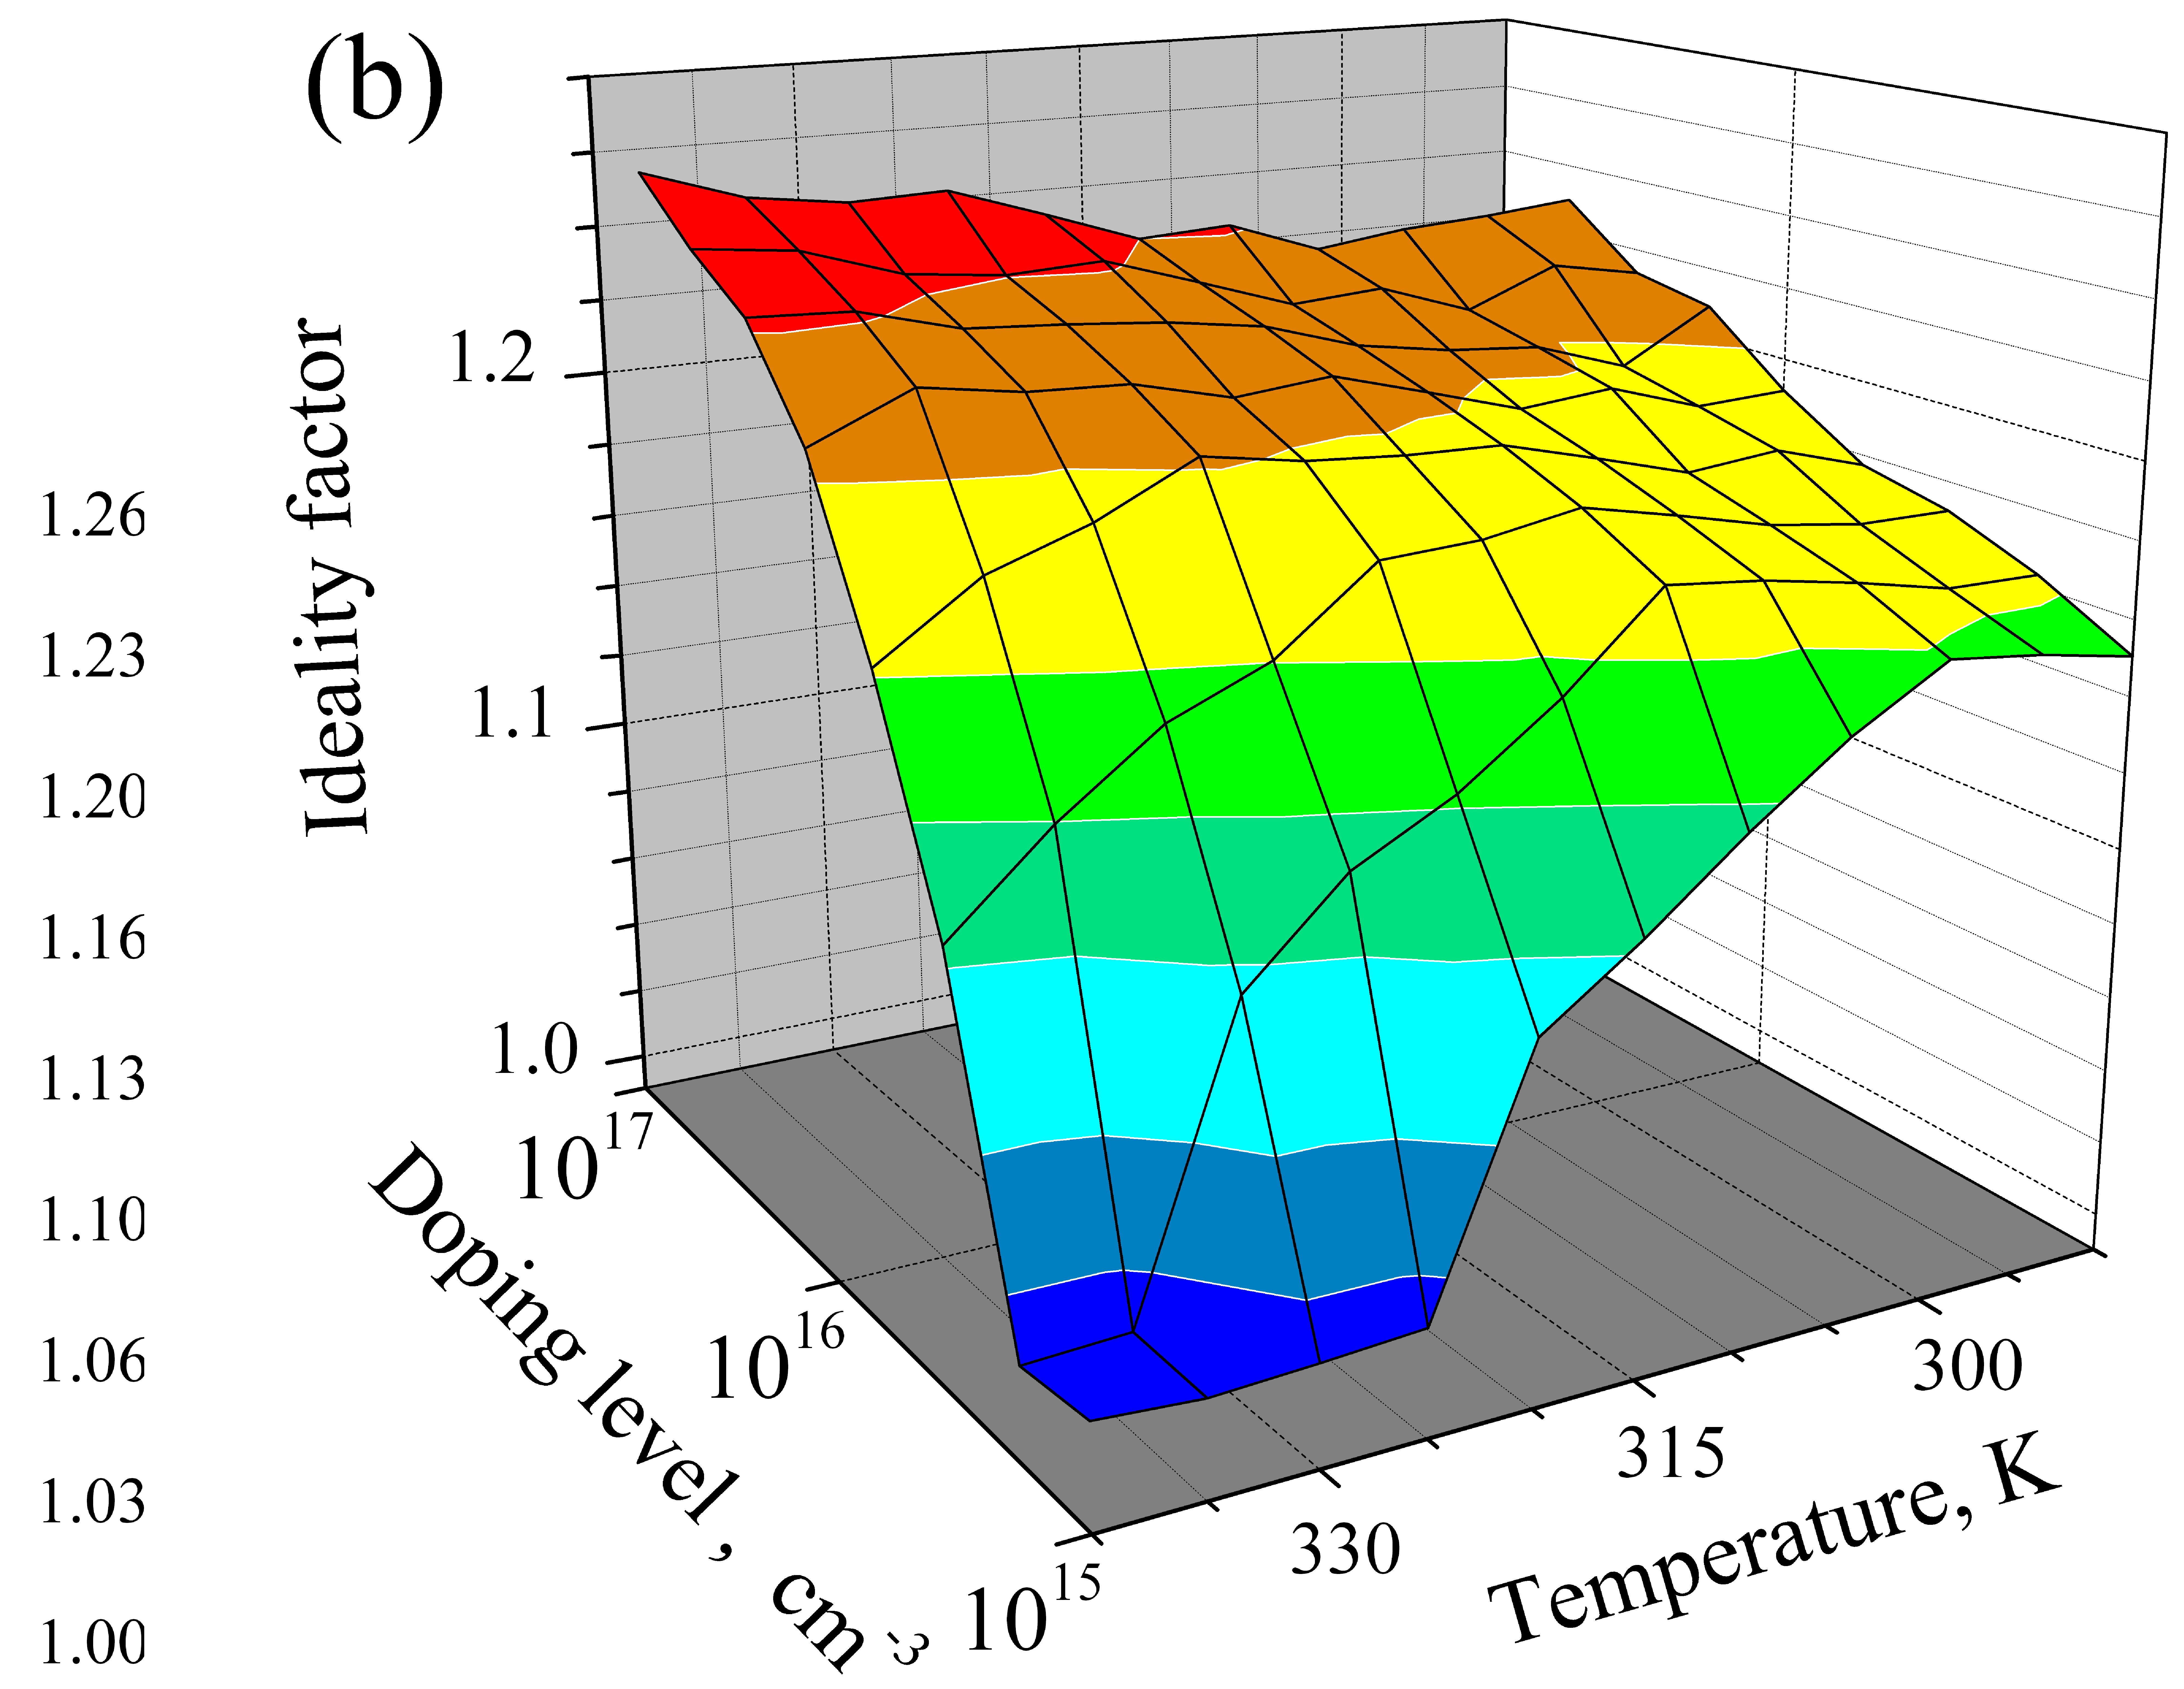
\includegraphics[width=0.5\textwidth]{Fig3b}
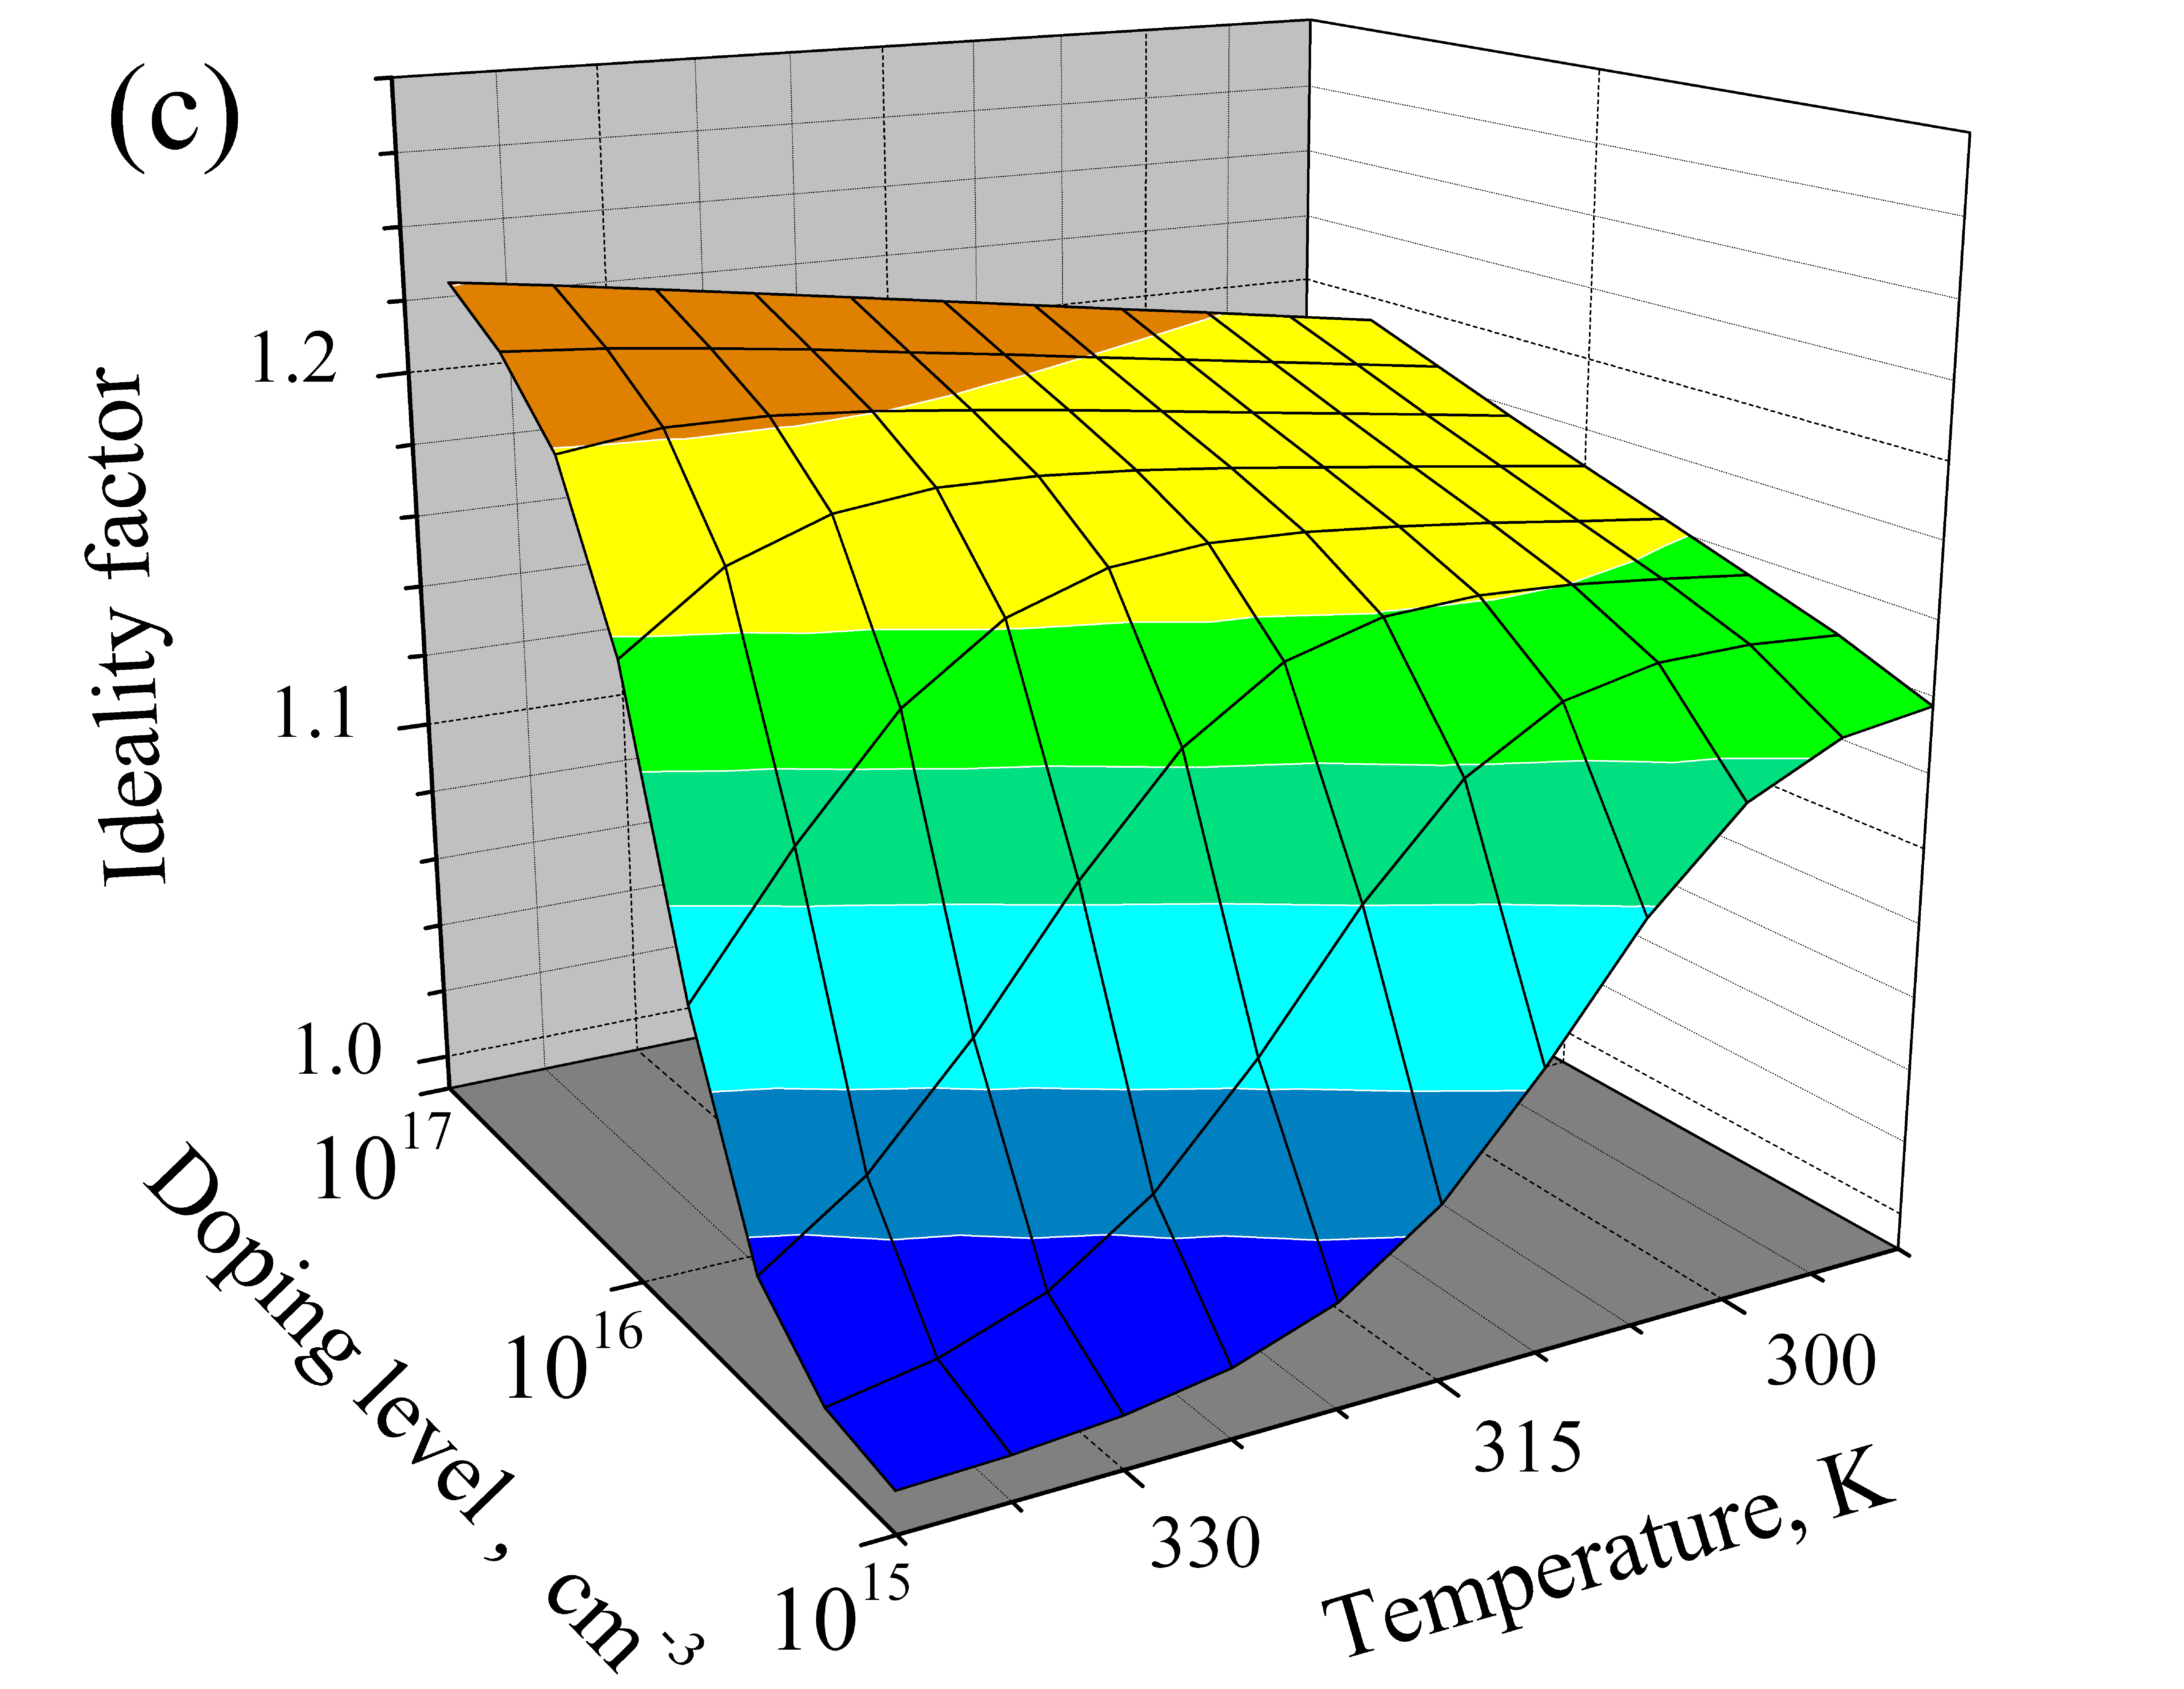
\includegraphics[width=0.5\textwidth]{Fig3c}

\includegraphics[width=0.5\textwidth]{Fig3d}
%\end{center}
\caption{\label{figA}
Ideality factor as a function of the temperature and dopant (boron) concentration.
FI--SRH case.
$N_\mathrm{Fe}$, cm$^{-3}$: $10^{10}$ (a,c), $10^{13}$ (b,d).
The simulated data are in panels (a) and (b);
the fittings of simulated data with help Eq.~(\ref{eqMain}) 
%and Table~\ref{tabEq} data 
are in panels (c) and (d).
}%
\end{figure}

It is clear that an analytical expression would be more convenient way to the $N_\mathrm{Fe}$ evaluation.
To build such expression one has to take into account that the interstitial iron captures an electron in $p$--type silicon.
Therefore the recombination affectivity is determined by a hole occurrence  on the $\mathrm{Fe}_i$ level.
The hole occupation probability is $f_p=\left[1+\exp\left(\frac{F-E_{\mathrm{Fe}_i}}{kT}\right)\right]^{-1}$ 
and this equation can be a start point to build an expression $n=n(T,N_\mathrm{A},N_\mathrm{Fe})$.
It must be considered that, unlike the simulated  $n(N_\mathrm{A},T)$ relationship,  
the $f_p(N_\mathrm{A},T)$ depends on temperature monotonically and reaches saturation with the increase in $N_\mathrm{A}$ --- one can see Supplementary Materials.
In addition, the Fermi level can be evaluated by the equation $F-E_V=kT\ln(N_V/N_\mathrm{A})$ under simulation conditions.

Based on aforesaid, we searched expression $n=n(T,N_\mathrm{A},N_\mathrm{Fe})$ in the following form:
\begin{equation}
\label{eqMain}
    n(T,N_\mathrm{A},N_\mathrm{Fe})=1+\frac{n_0(N_\mathrm{Fe})\cdot T^{m_T}\cdot(\log N_\mathrm{A})^{m_\mathrm{A}}}
        {1+N_V(T)\cdot\gamma(N_\mathrm{A},N_\mathrm{Fe})\cdot\exp\left(\frac{E_\mathrm{ef}(T,N_\mathrm{A})}{kT}\right)}\,,
\end{equation}
where 
$m_T$ and $m_\mathrm{A}$ are the constant,
and fitness parameters $n_0$, $\gamma$, and $E_\mathrm{ef}$ depend on iron concentration, doping level, and temperature.

The analysis has shown that the simulated data are well fitted by Eq.~(\ref{eqMain}) with $m_T=1.13$, $m_\mathrm{A}=2.85$, $\gamma=N_\mathrm{A}^{-1}$.
Besides the dependence of the effective energy $E_\mathrm{ef}$ can be expressed as:
\begin{equation}
\label{eqEf-FISRH}
    E_\mathrm{ef}(T,N_\mathrm{A})=E_0-\alpha\, T / \log N_\mathrm{A}+\beta \,T\,,
\end{equation}
where
values $E_0=1.43\pm0.08$~eV, $\alpha=85\pm5$~meV$\,$cm$^{-3}$K$^{-1}$, and $\beta=1.9\pm0.2$~meV$\,$K$^{-1}$ do not depend on $N_\mathrm{Fe}$ practically.
The parameters are listed in Table~\ref{tabEq} and the results of the fitting are shown in Fig.~\ref{figA}(c,d), and Supplementary Materials.  
A good agreement of  simulated data and fitting curves prove the expediency of Eq.~(\ref{eqMain}) using.
%
%\begin{table}
%\caption{\label{tabEq}Parameters of Eq.~(\ref{eqMain}) fitting of simulated ideality factor relationships.
%}
%\begin{tabular}{lcccc}
%\hline
%\hline
%Parameter&\multicolumn{4}{c}{Simulation case}\\
%&FI--SRH&FI--SRHBBA&FIFB--SRH&FIFB--SRHBBA\\
%\hline
%$m_T$&1.13&1.3&2.2&2.2\\
%$m_\mathrm{A}$&2.85&2.85&2.85&2.85\\
%$\gamma$&$N_\mathrm{A}^{-1}$&Eq.~(\ref{eqGamma}), Fig.~\ref{fig7}(a)&Fig.~\ref{fig9}(a)&Fig.~\ref{fig9}(b)\\
%$E_\mathrm{ef}$, eV&$1.43-\frac{0.085\, T} {\log N_\mathrm{A}}+0.0019 \,T$&$9.53-0.52\log N_\mathrm{A}$&$16.6-0.90\log N_\mathrm{A}$&$13.4-0.77\log N_\mathrm{A}$\\
%$n_0$&Eq.~(\ref{eqN0}), Fig.~\ref{fig4}&Fig.~\ref{fig7}(b)&Fig.~\ref{fig10}(a)&Fig.~\ref{fig10}(b)\\
%\hline
%\hline
%\end{tabular}
%\end{table}


%\begin{table}
%\caption{\label{tabEq}Parameters of Eq.~(\ref{eqMain}) fitting of simulated ideality factor relationships.
%}
%\begin{tabular}{lccccc}
%\hline
%\hline
%Simulation case&\multicolumn{5}{c}{Parameter}\\
%&$m_T$&$m_\mathrm{A}$&$\gamma$&$E_\mathrm{ef}$, eV&$n_0$\\
%\hline
%FI--SRH&1.13&2.85&$N_\mathrm{A}^{-1}$&$1.43-\frac{0.085\, T} {\log N_\mathrm{A}}+0.0019 \,T$&Eq.~(\ref{eqN0}), Fig.~\ref{fig4}\\
%FI--SRHBBA&1.3&2.85&Eq.~(\ref{eqGamma}), Fig.~\ref{fig7}(a)&$9.53-0.52\log N_\mathrm{A}$&Fig.~\ref{fig7}(b)\\
%FIFB--SRH&2.2&2.85&Fig.~\ref{fig9}(a)&$16.6-0.90\log N_\mathrm{A}$&Fig.~\ref{fig10}(a)\\
%FIFB--SRHBBA&2.2&2.85&Fig.~\ref{fig9}(b)&$13.4-0.77\log N_\mathrm{A}$&Fig.~\ref{fig10}(b)\\
%\hline
%\hline
%\end{tabular}
%\end{table}

\begin{table}
\caption{\label{tabEq}Parameters of Eq.~(\ref{eqMain}) fitting of simulated ideality factor relationships.
}
\begin{tabular}{lcccc}
\hline
\hline
Simulation case&\multicolumn{4}{c}{Parameter}\\
&$m_T$&$m_\mathrm{A}$&$\gamma$&$E_\mathrm{ef}$, eV\\
\hline
FI--SRH&1.13&2.85&$N_\mathrm{A}^{-1}$&$1.43-\frac{0.085\, T} {\log N_\mathrm{A}}+0.0019 \,T$\\
FI--SRHBBA&1.3&2.85&Eq.~(\ref{eqGamma})&$9.53-0.52\log N_\mathrm{A}$\\
FIFB--SRH&2.2&2.85&Fig.~\ref{fig9}(a)&$16.6-0.90\log N_\mathrm{A}$\\
FIFB--SRHBBA&2.2&2.85&Fig.~\ref{fig9}(b)&$13.4-0.77\log N_\mathrm{A}$\\
\hline
\hline
\end{tabular}
\end{table}


Thus, in the FI--SRH case, the simulated (semi--empirical) dependence of the ideality factor takes the following shape:
\begin{equation}
\label{eqM-FISRH}
    n=1+\frac{n_0(N_\mathrm{Fe})\cdot T^{1.13}\cdot(\log N_\mathrm{A})^{2.85}}
        {1+\frac{N_V(T)}{N_\mathrm{A}}\cdot\exp\left(\frac{1.43}{kT}-\frac{986}{\log N_\mathrm{A}}+22\right)}\,.
\end{equation}

We use Eq.~(\ref{eqM-FISRH}) by taking $n_0$ as fitting parameter to fit the $n$ dependencies, calculated for different $N_\mathrm{Fe}$ value.
The resulting $n_0$ dependence on iron concentration is shown in Fig.~\ref{fig4}.
This curve is monotonic as well as  smooth enough and can serves as a calibration curve.
In addition, the found dependence is well described by Eq.~(\ref{eqN0}):
\begin{equation}
\label{eqN0}
    n_0(N_\mathrm{Fe})=1.28\times10^{-7}-\frac{2.38\times10^{-8}}{1+\left(\frac{N_\mathrm{Fe}}{4.96\times10^{12}}\right)^{0.85}}\,.
\end{equation}

\begin{figure}
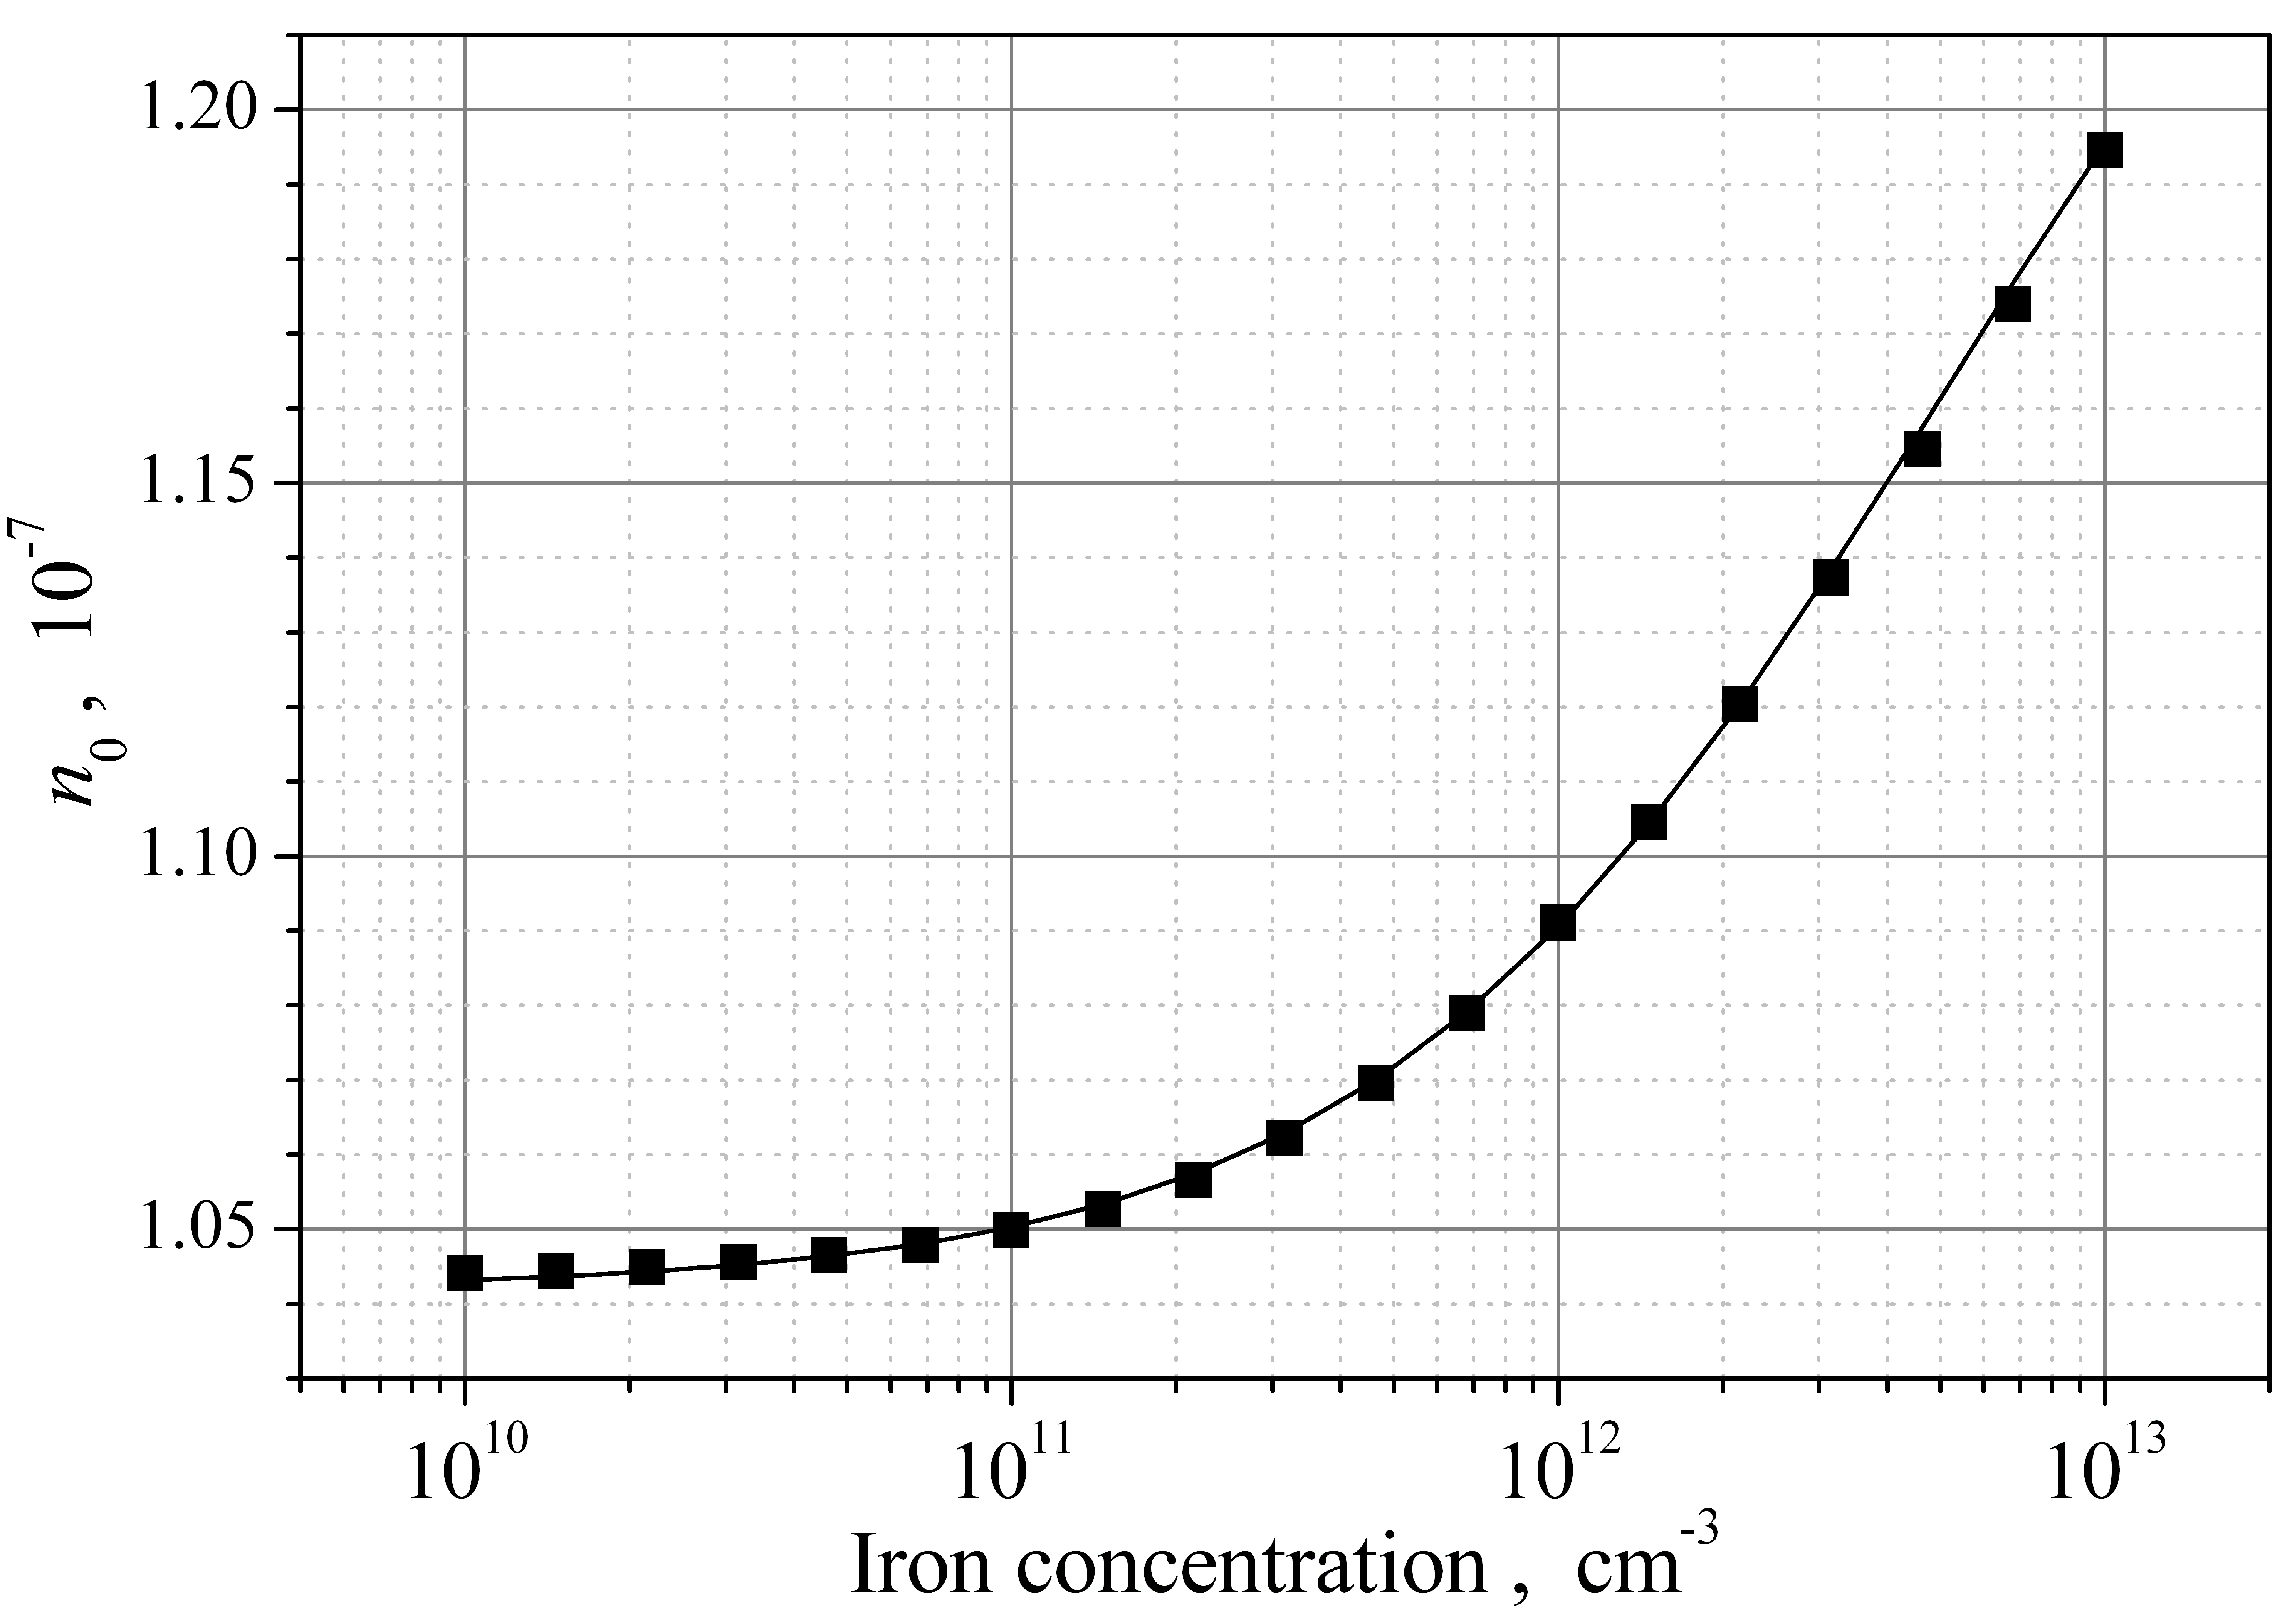
\includegraphics[width=0.6\textwidth]{Fig4}%
\caption{\label{fig4}
Dependence of the parameter $n_0$ (see Eq.~(\ref{eqMain})) on the iron concentration in SC base.
FI--SRH case.
Line is the fitted curve using Eq.~(\ref{eqN0}).
}%
\end{figure}

Thus, the algorithm of an iron concentration evaluation in a silicon SC by using $I-V$ curve can be as following.
\begin{enumerate}[(i)]
\item The solar cell is illuminated by 15 to 90 s with a halogen lamp to dissociate the FeB pairs.
      When illumination stopped, the $I-V$ curve is measured.
\item $I-V$ curve is fitted accordingly to the two--diode model and the ideality factor $n$ is determined.
\item Taking into account $n$ value, doping level $N_\mathrm{A}$, and measurement temperature,
      the parameter $n_0$ is calculated by relationship
\begin{displaymath}
    n_0=(n-1)\cdot \frac{1+\frac{N_V(T)}{N_\mathrm{A}}\cdot\exp\left(\frac{1.43}{kT}-\frac{986}{\log N_\mathrm{A}}+22\right)}{T^{1.13}\cdot(\log N_\mathrm{A})^{2.85}}\,.
\end{displaymath}
\item $N_\mathrm{Fe}$ is evaluated by using calibration curve in Fig.~\ref{eqN0} or by relationship
\begin{displaymath}
    N_\mathrm{Fe}=4.96\times10^{12}\cdot \left(\frac{2.38\times10^{-8}}{1.28\times10^{-7}-n_0}\right)^{1.18}\,.
\end{displaymath}
\end{enumerate}


\subsection{Interstitial iron, SRH and intrinsic recombination}




\begin{figure}
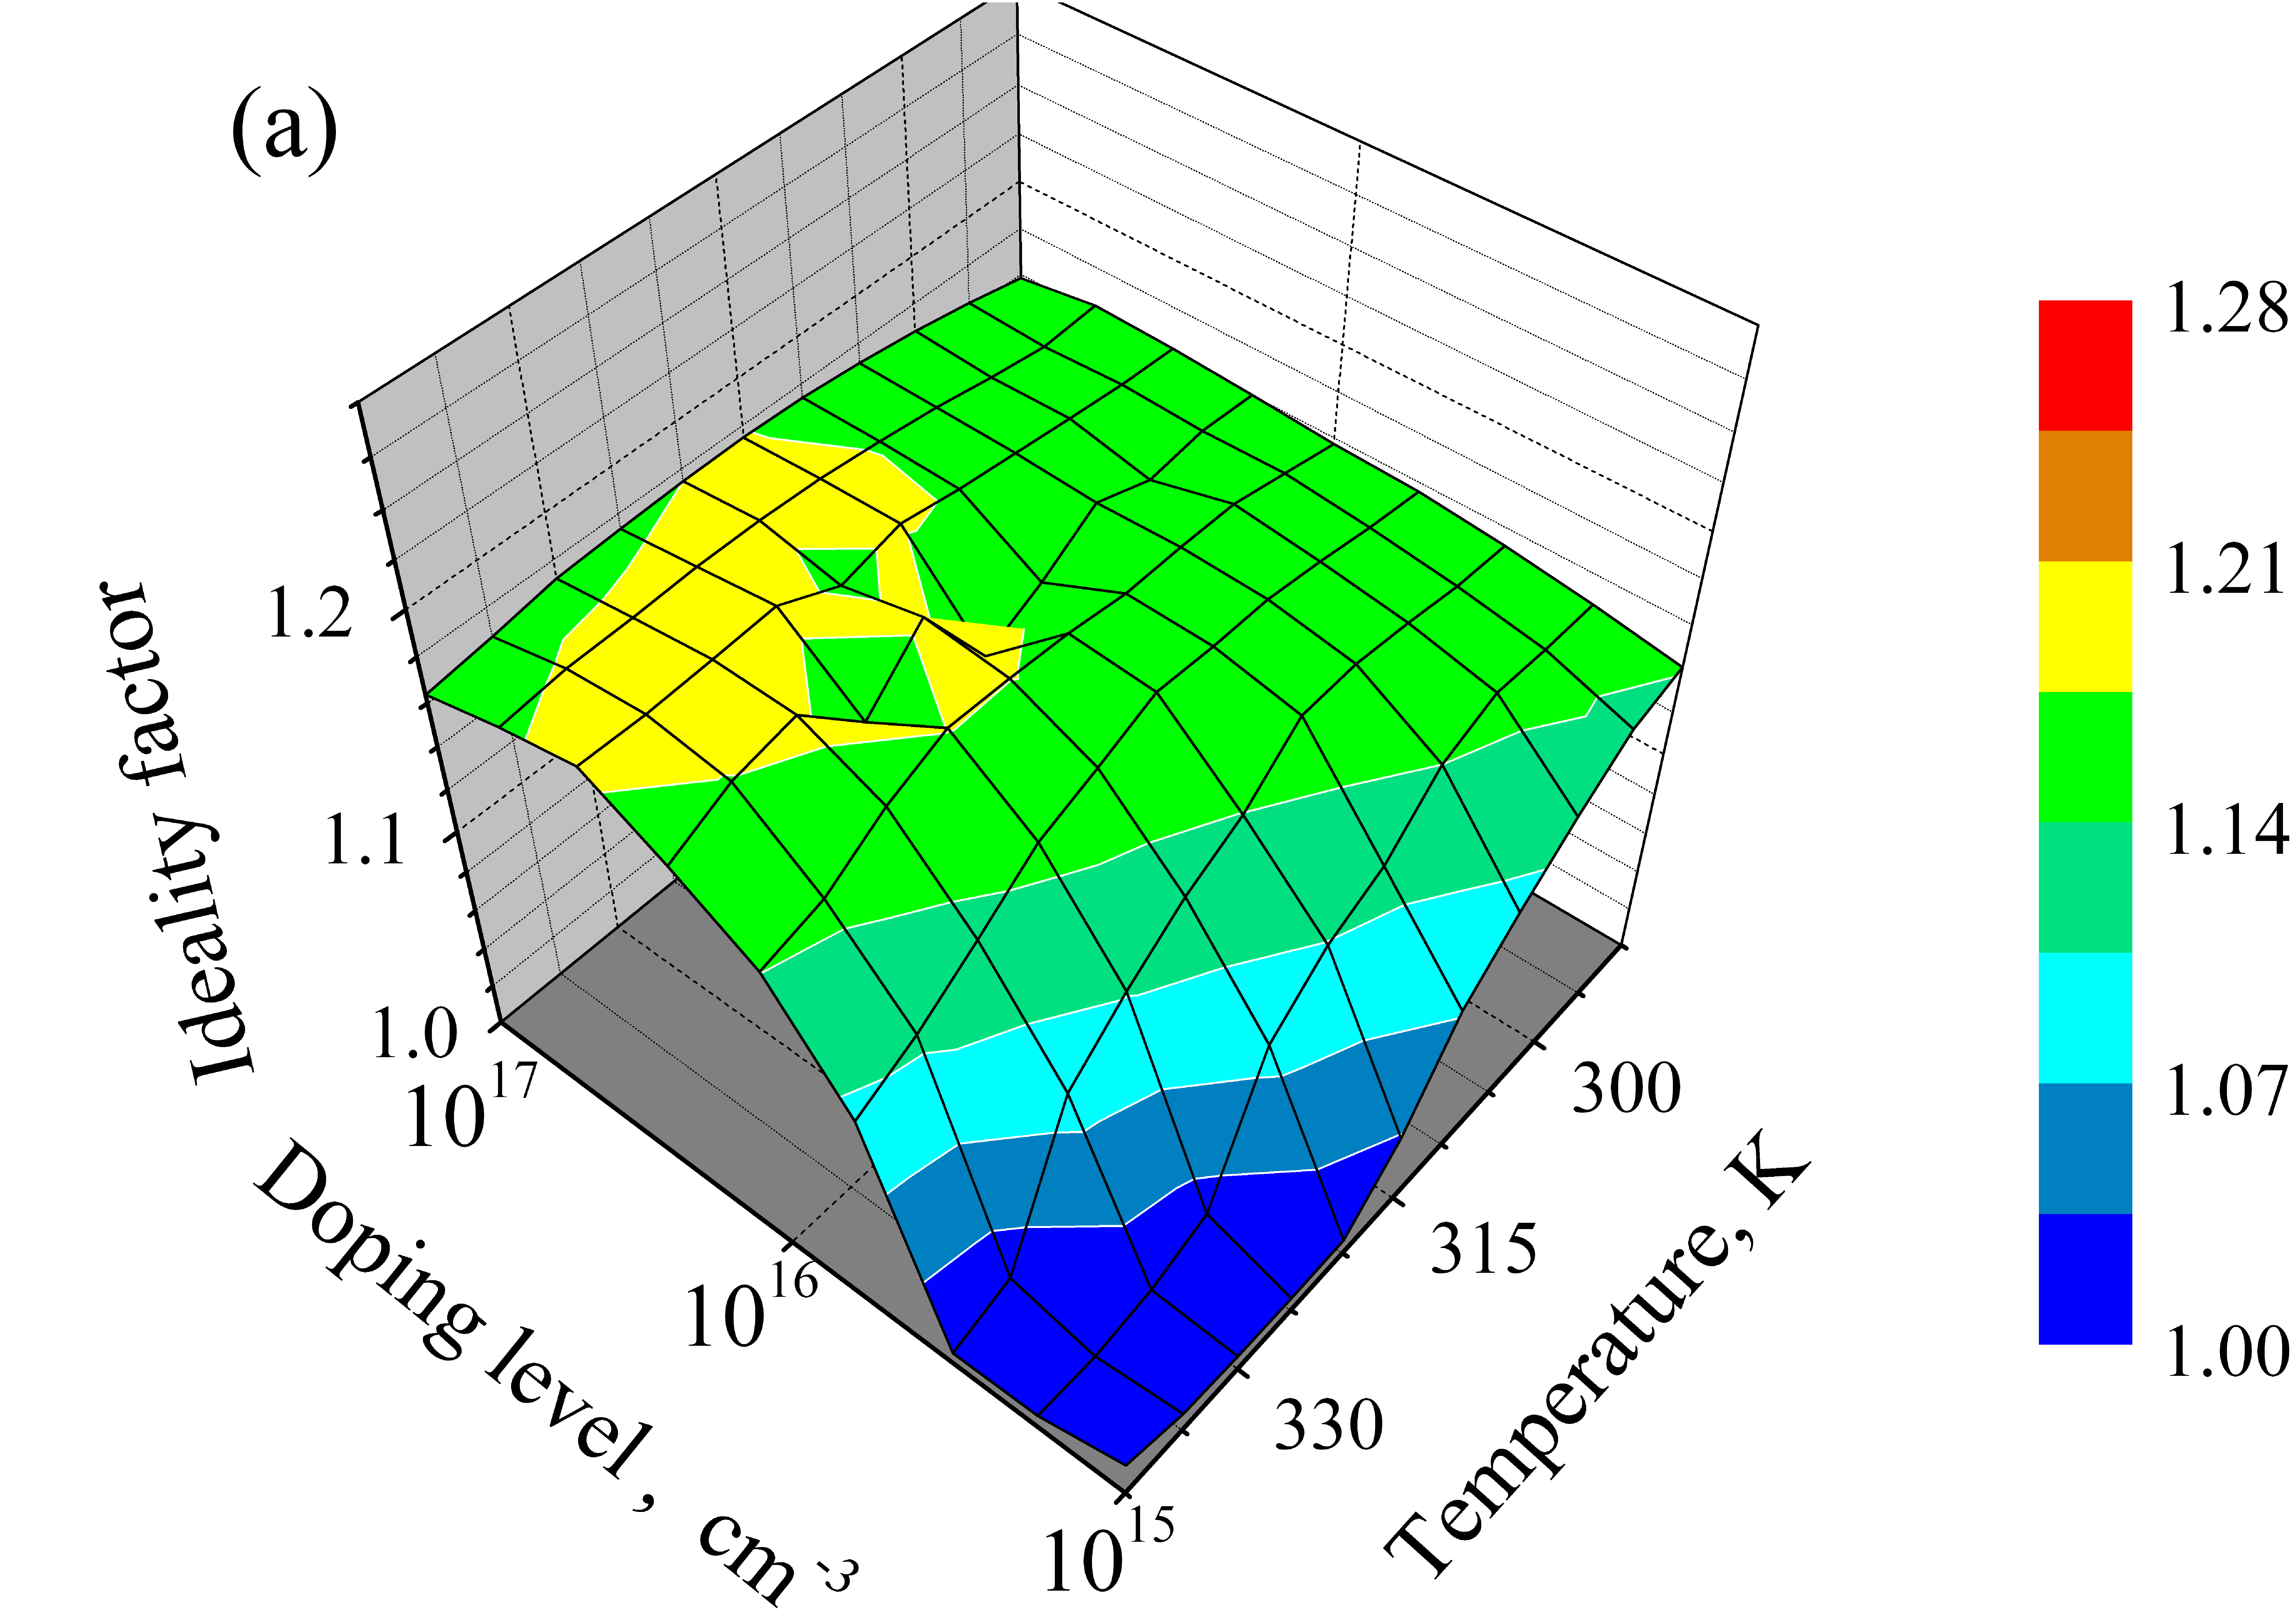
\includegraphics[width=0.5\textwidth]{Fig5a}%
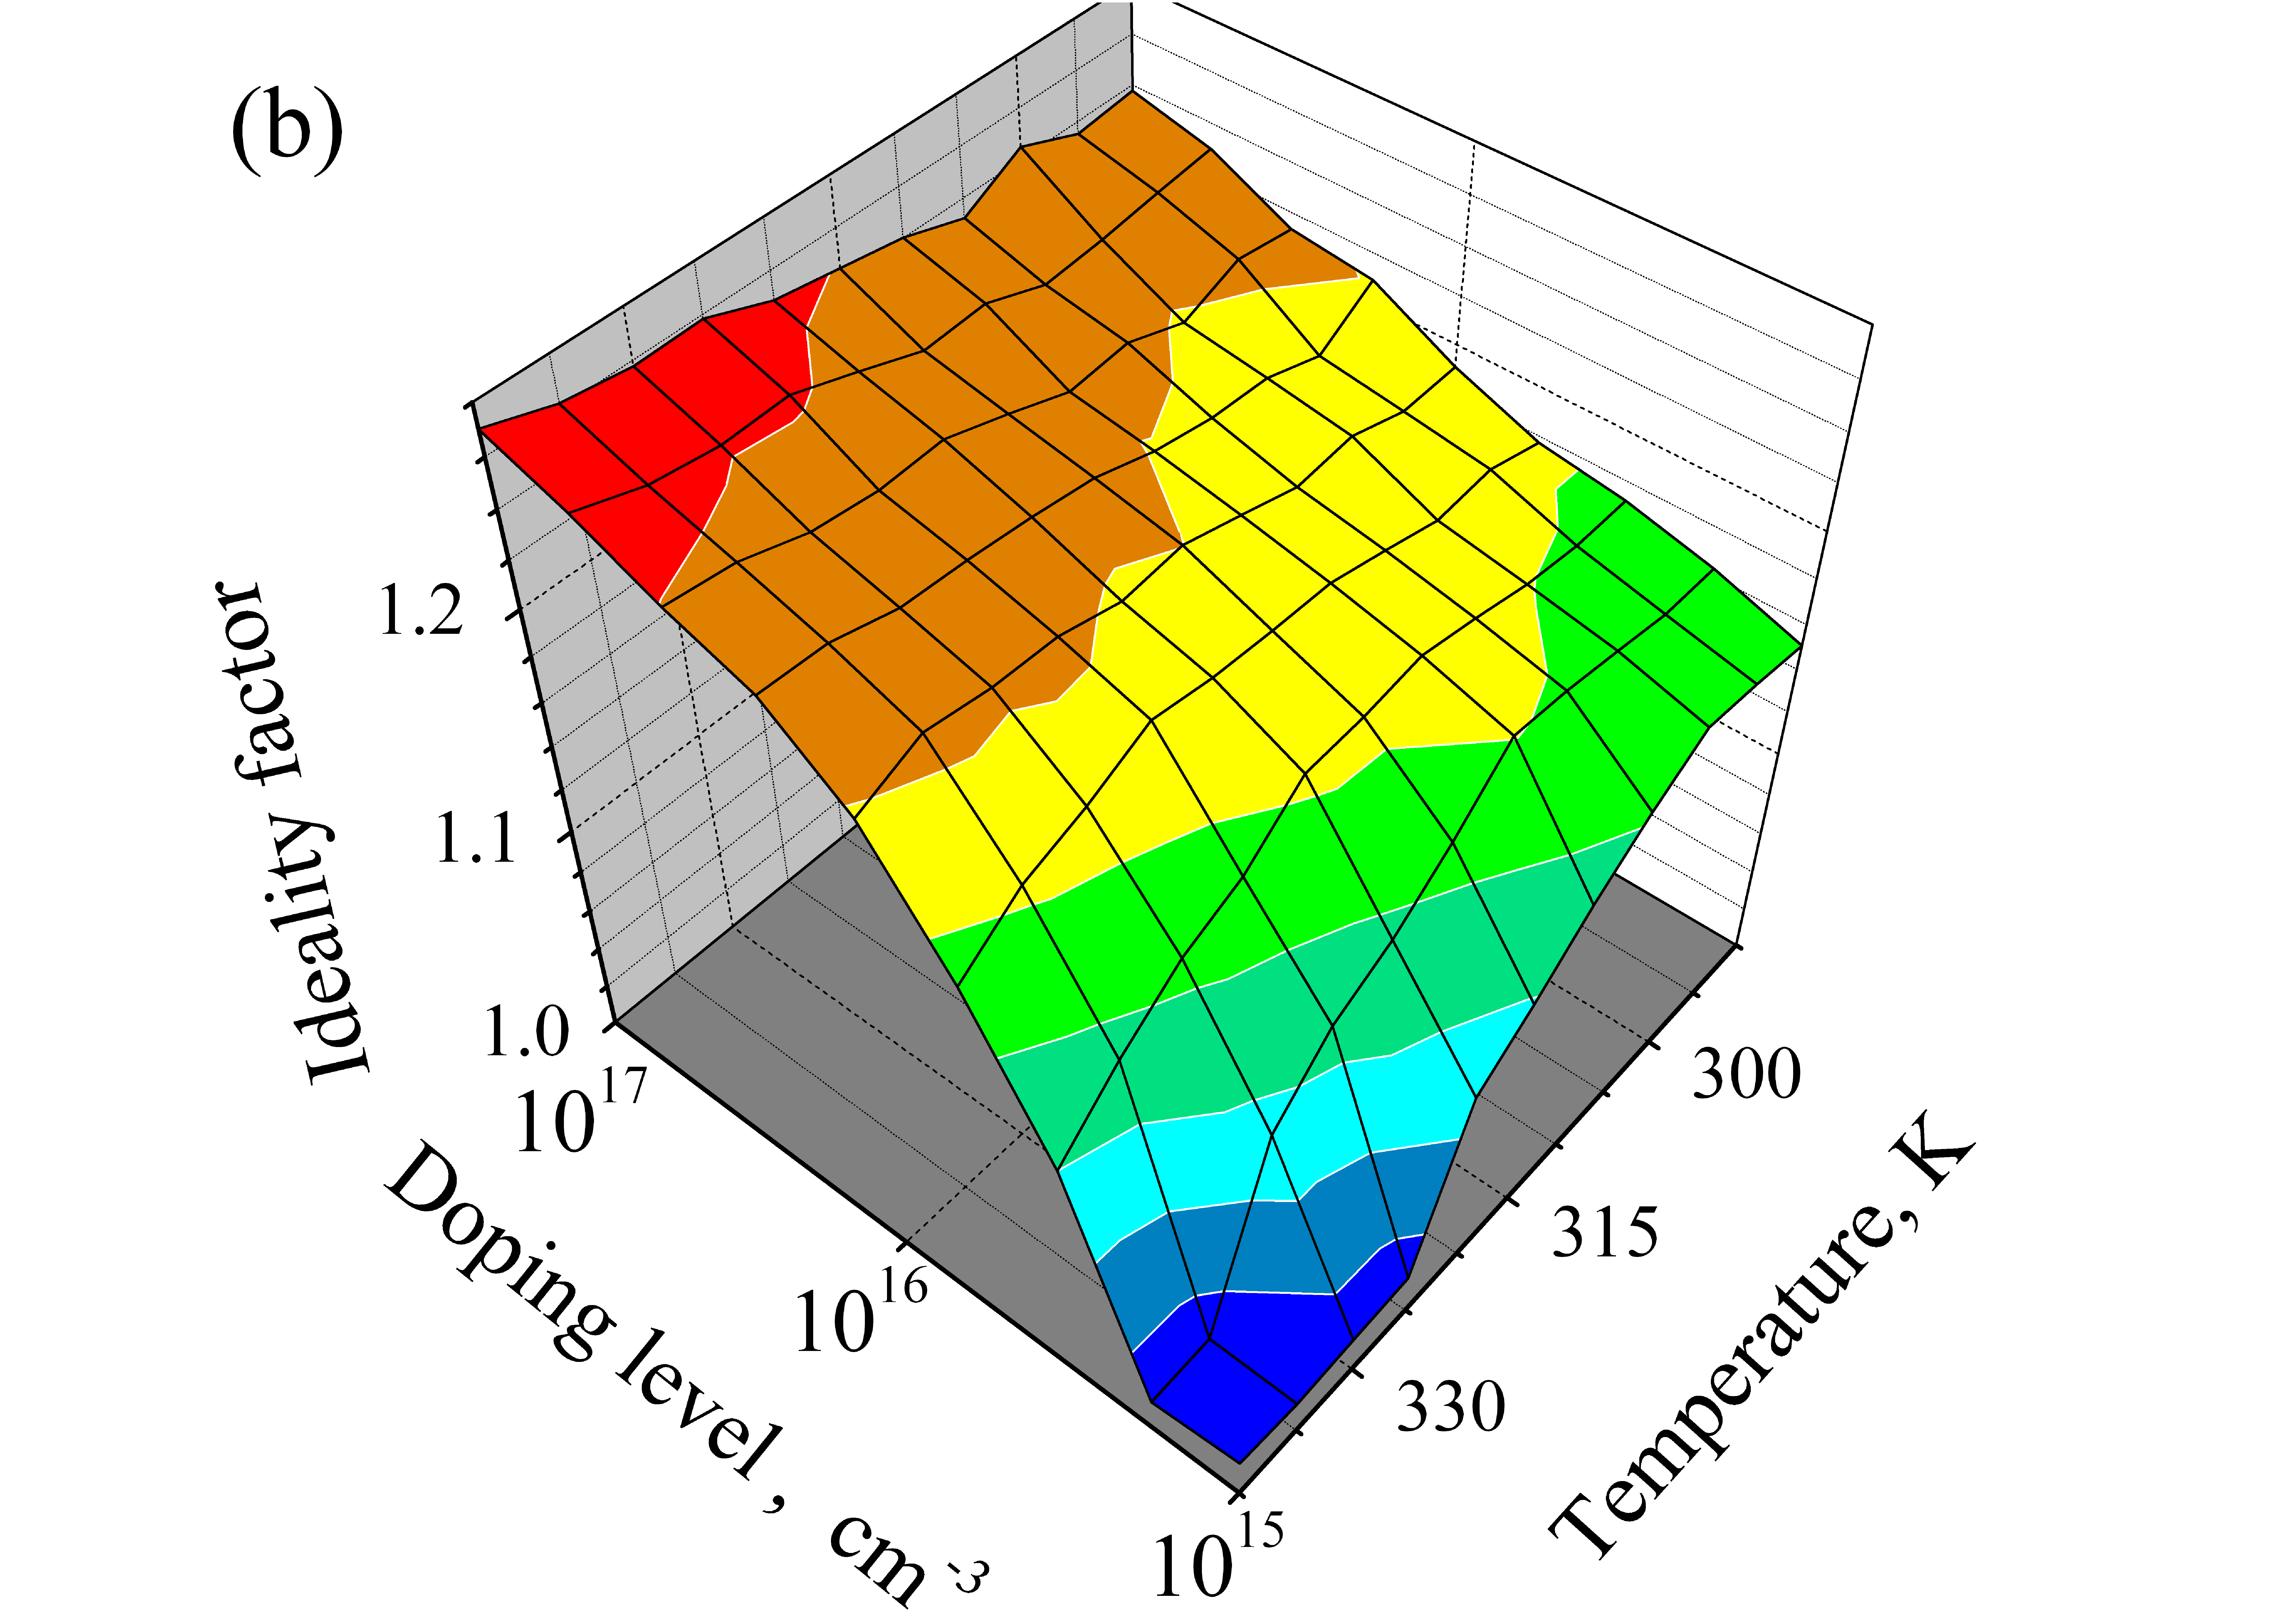
\includegraphics[width=0.5\textwidth]{Fig5b}
\caption{\label{fig5}
Ideality factor as a function of the temperature and dopant (boron) concentration.
FI--SRHBBA case.
$N_\mathrm{Fe}$, cm$^{-3}$: $10^{10}$ (a), $10^{13}$ (b).
}%
\end{figure}


\begin{equation}
\label{eqGamma}
    \gamma=\left(\frac{10^{15}}{N_\mathrm{A}}\right)^{11}\cdot \frac{\eta N_0+N_\mathrm{Fe}}{N_0+N_\mathrm{Fe}}\,.
\end{equation}


\begin{figure}
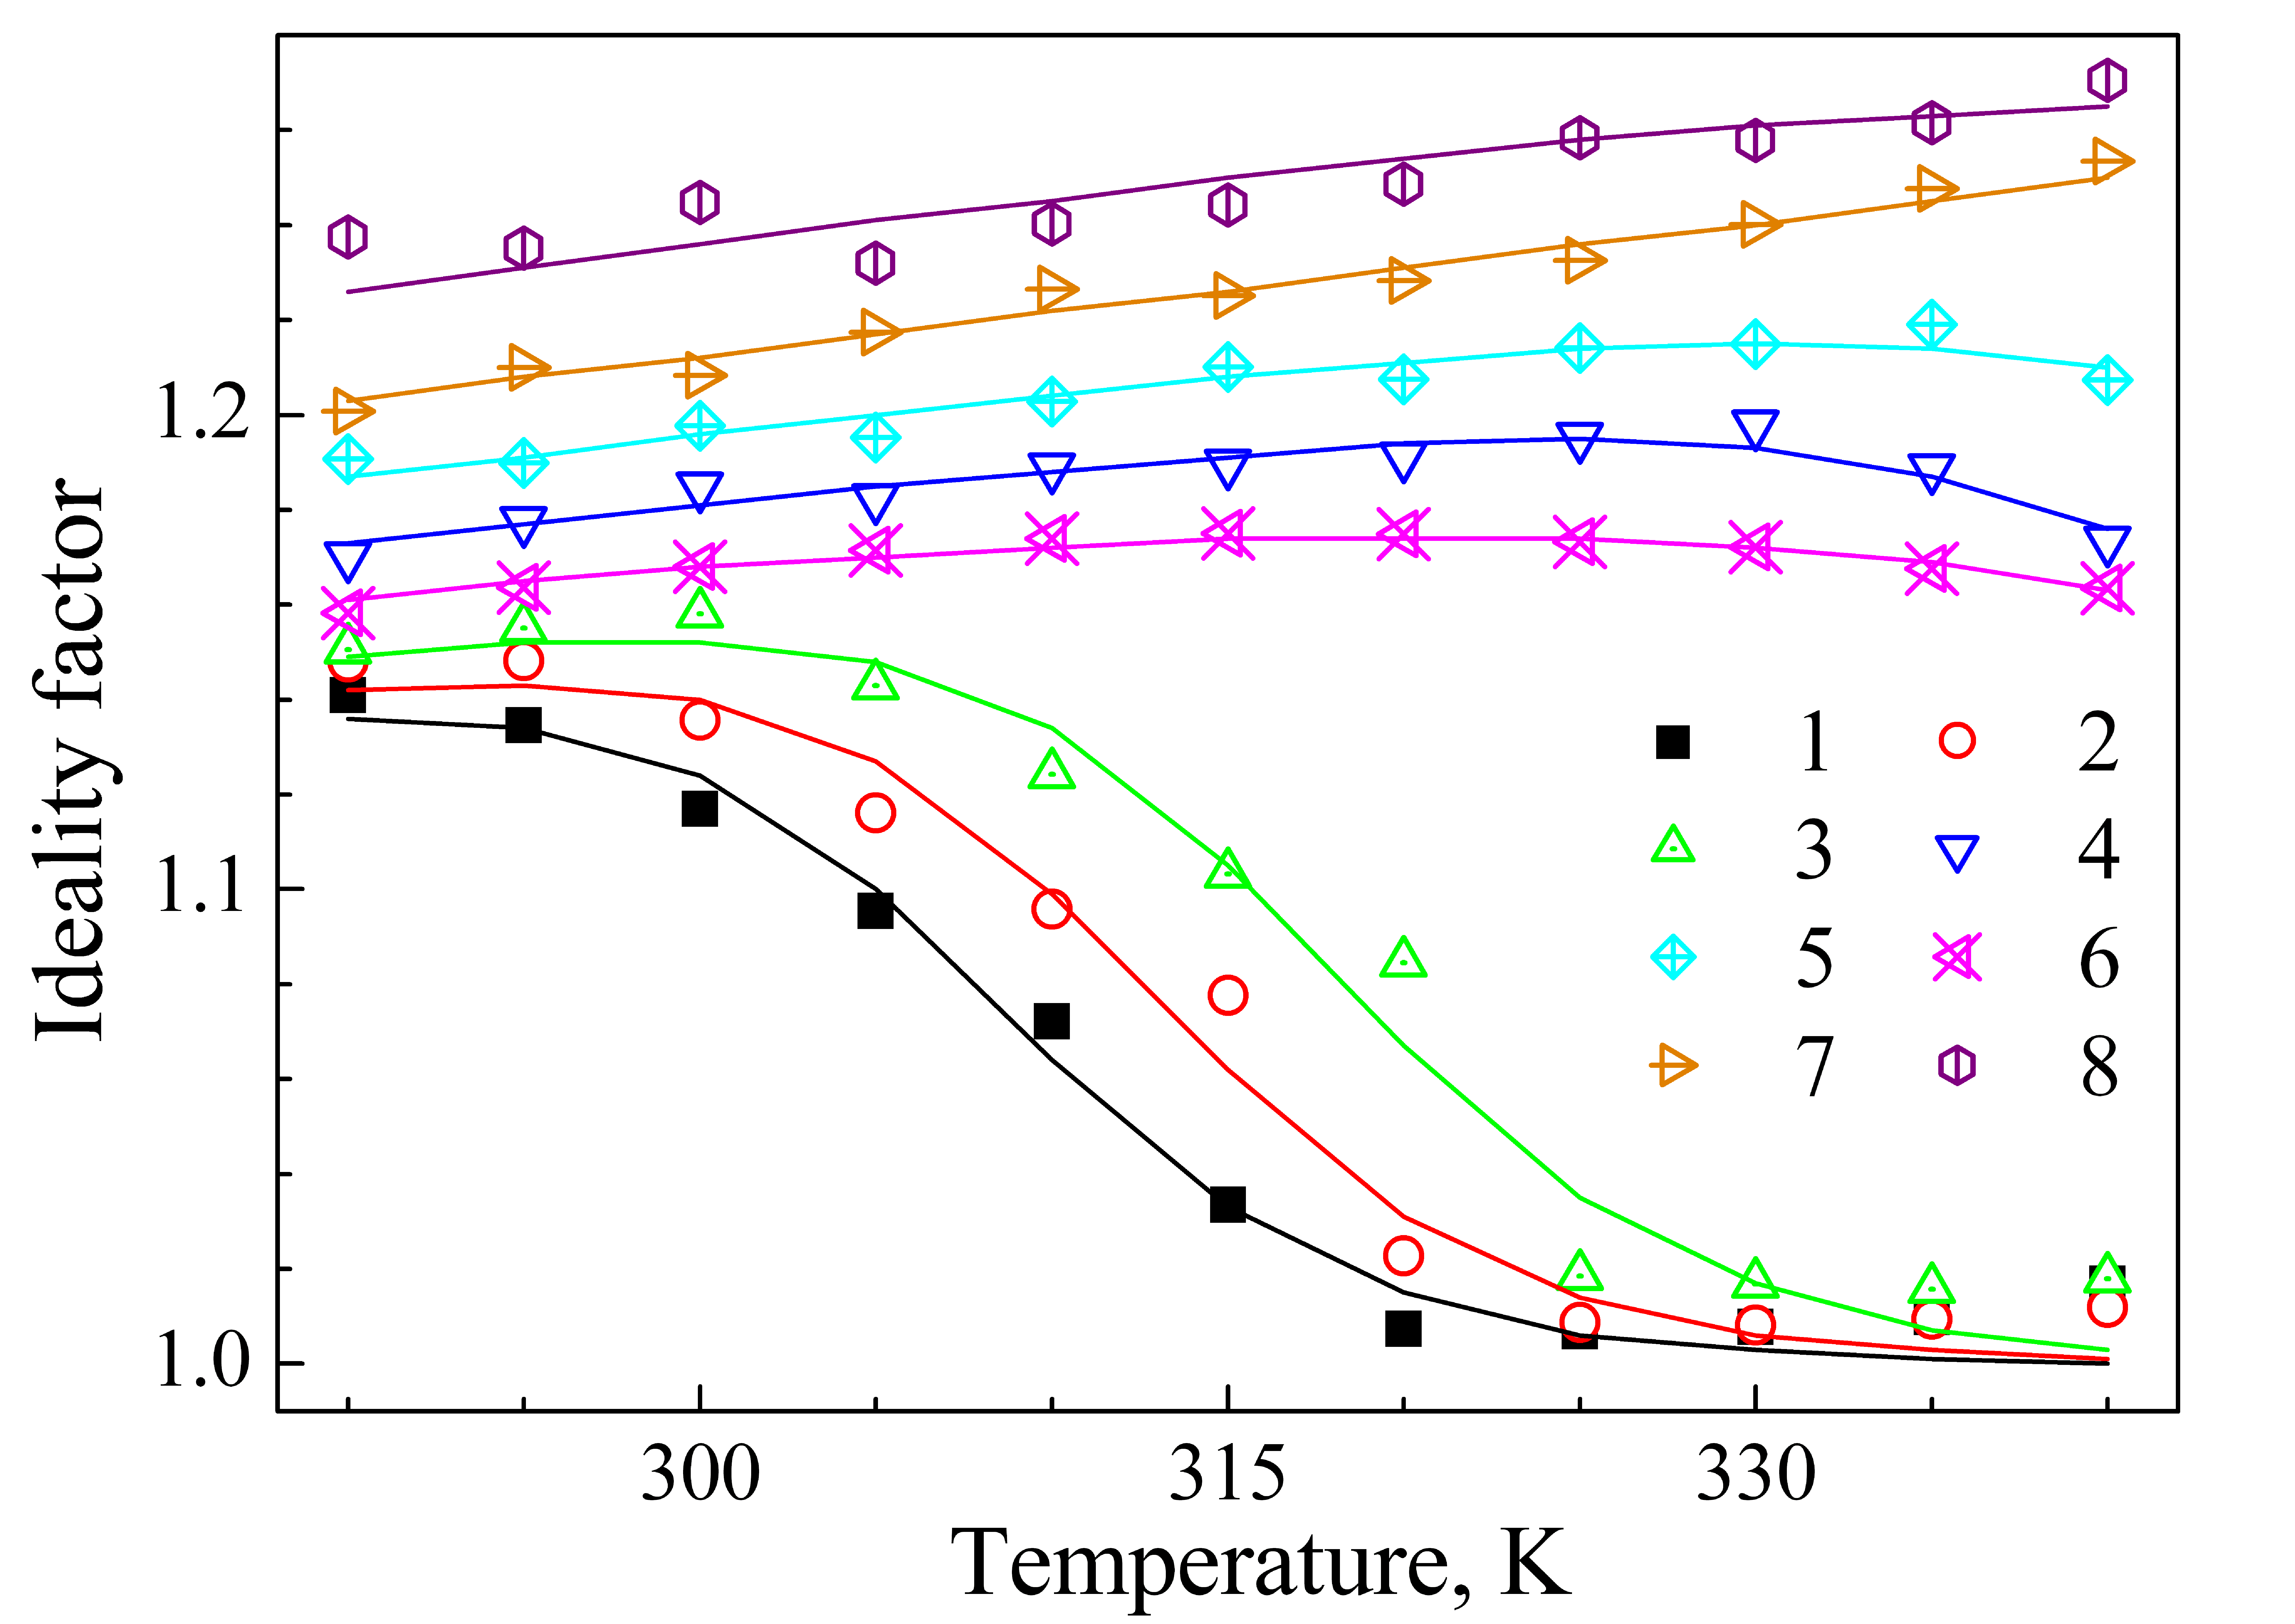
\includegraphics[width=0.6\textwidth]{Fig6}%
\caption{\label{fig6}
Temperature dependencies of the ideality factor.
FI--SRHBBA case.
The marks are the simulation results, and the lines are the fitted curves using Eq.~(\ref{eqMain}) and data in Table~\ref{tabEq}.
$N_\mathrm{Fe}$, cm$^{-3}$: $10^{10}$ (curves 1, 6), $10^{12}$ (2, 4, and 7), $10^{13}$ (3, 5, and 8).
$N_\mathrm{A}$ cm$^{-3}$: $10^{15}$ (1, 2, and 3), $10^{16}$ (4,  5), $10^{17}$ (6, 7, and 8).
}%
\end{figure}

\begin{figure}
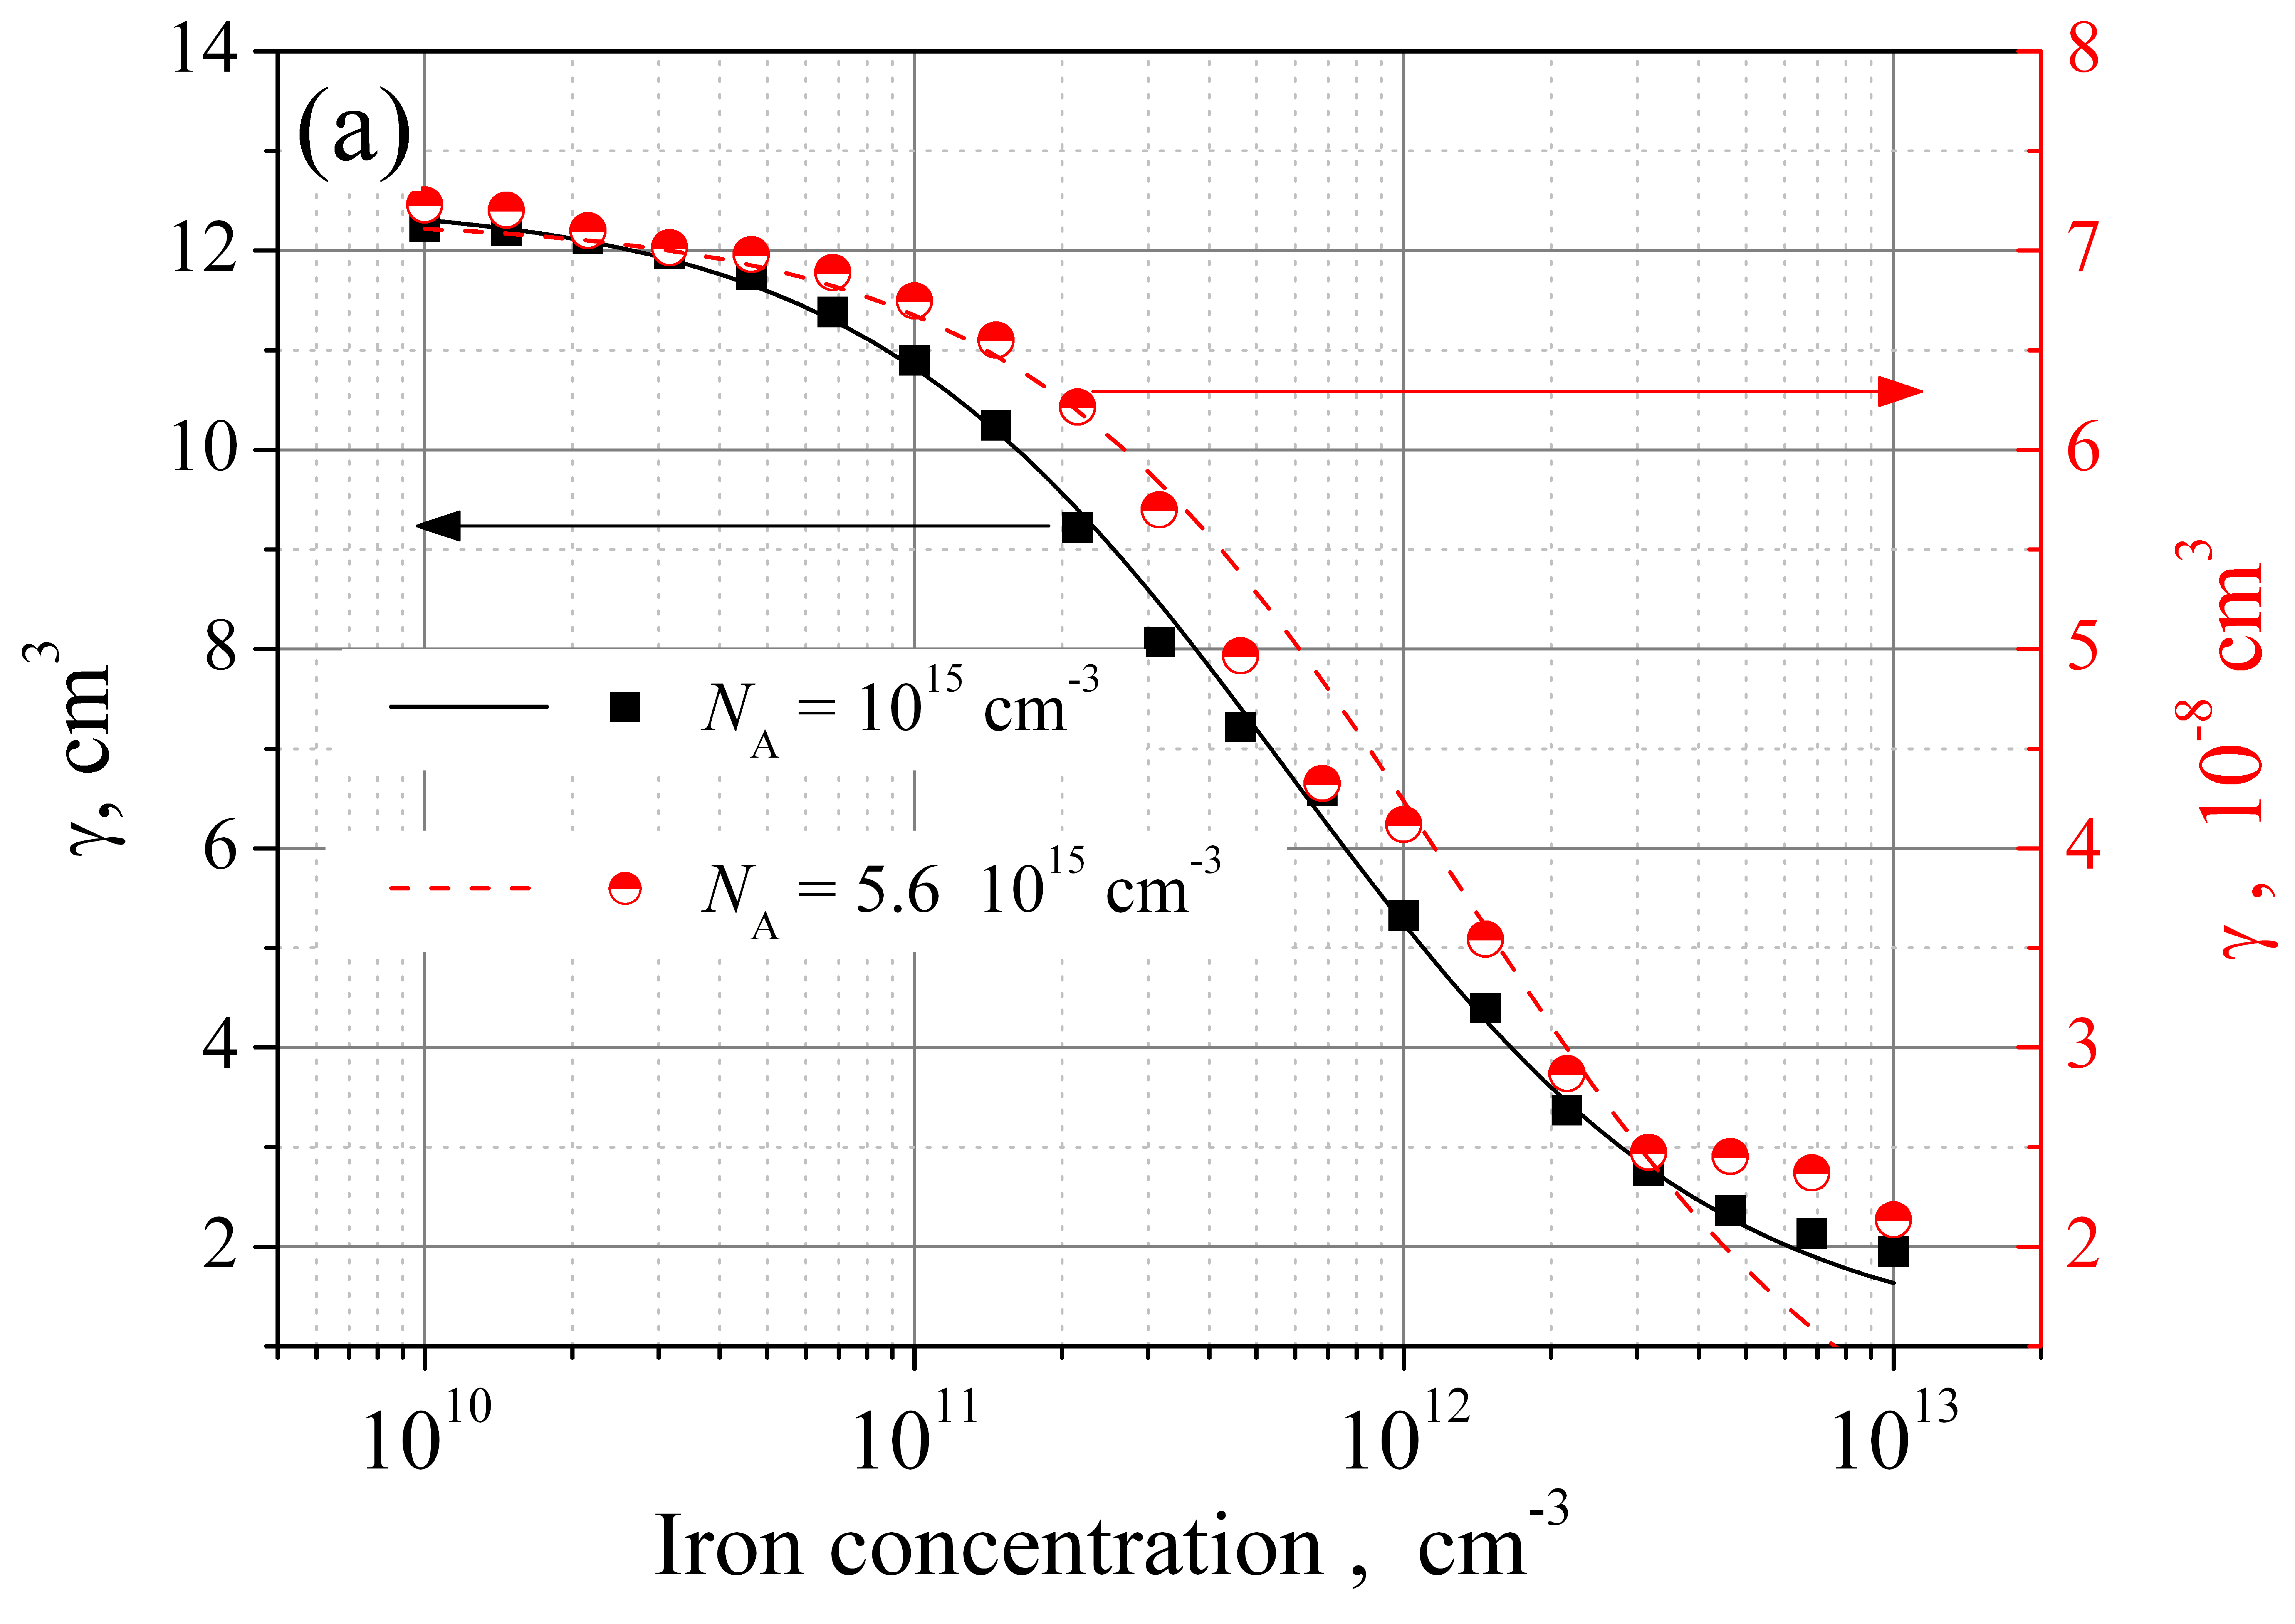
\includegraphics[width=0.5\textwidth]{Fig7a}%
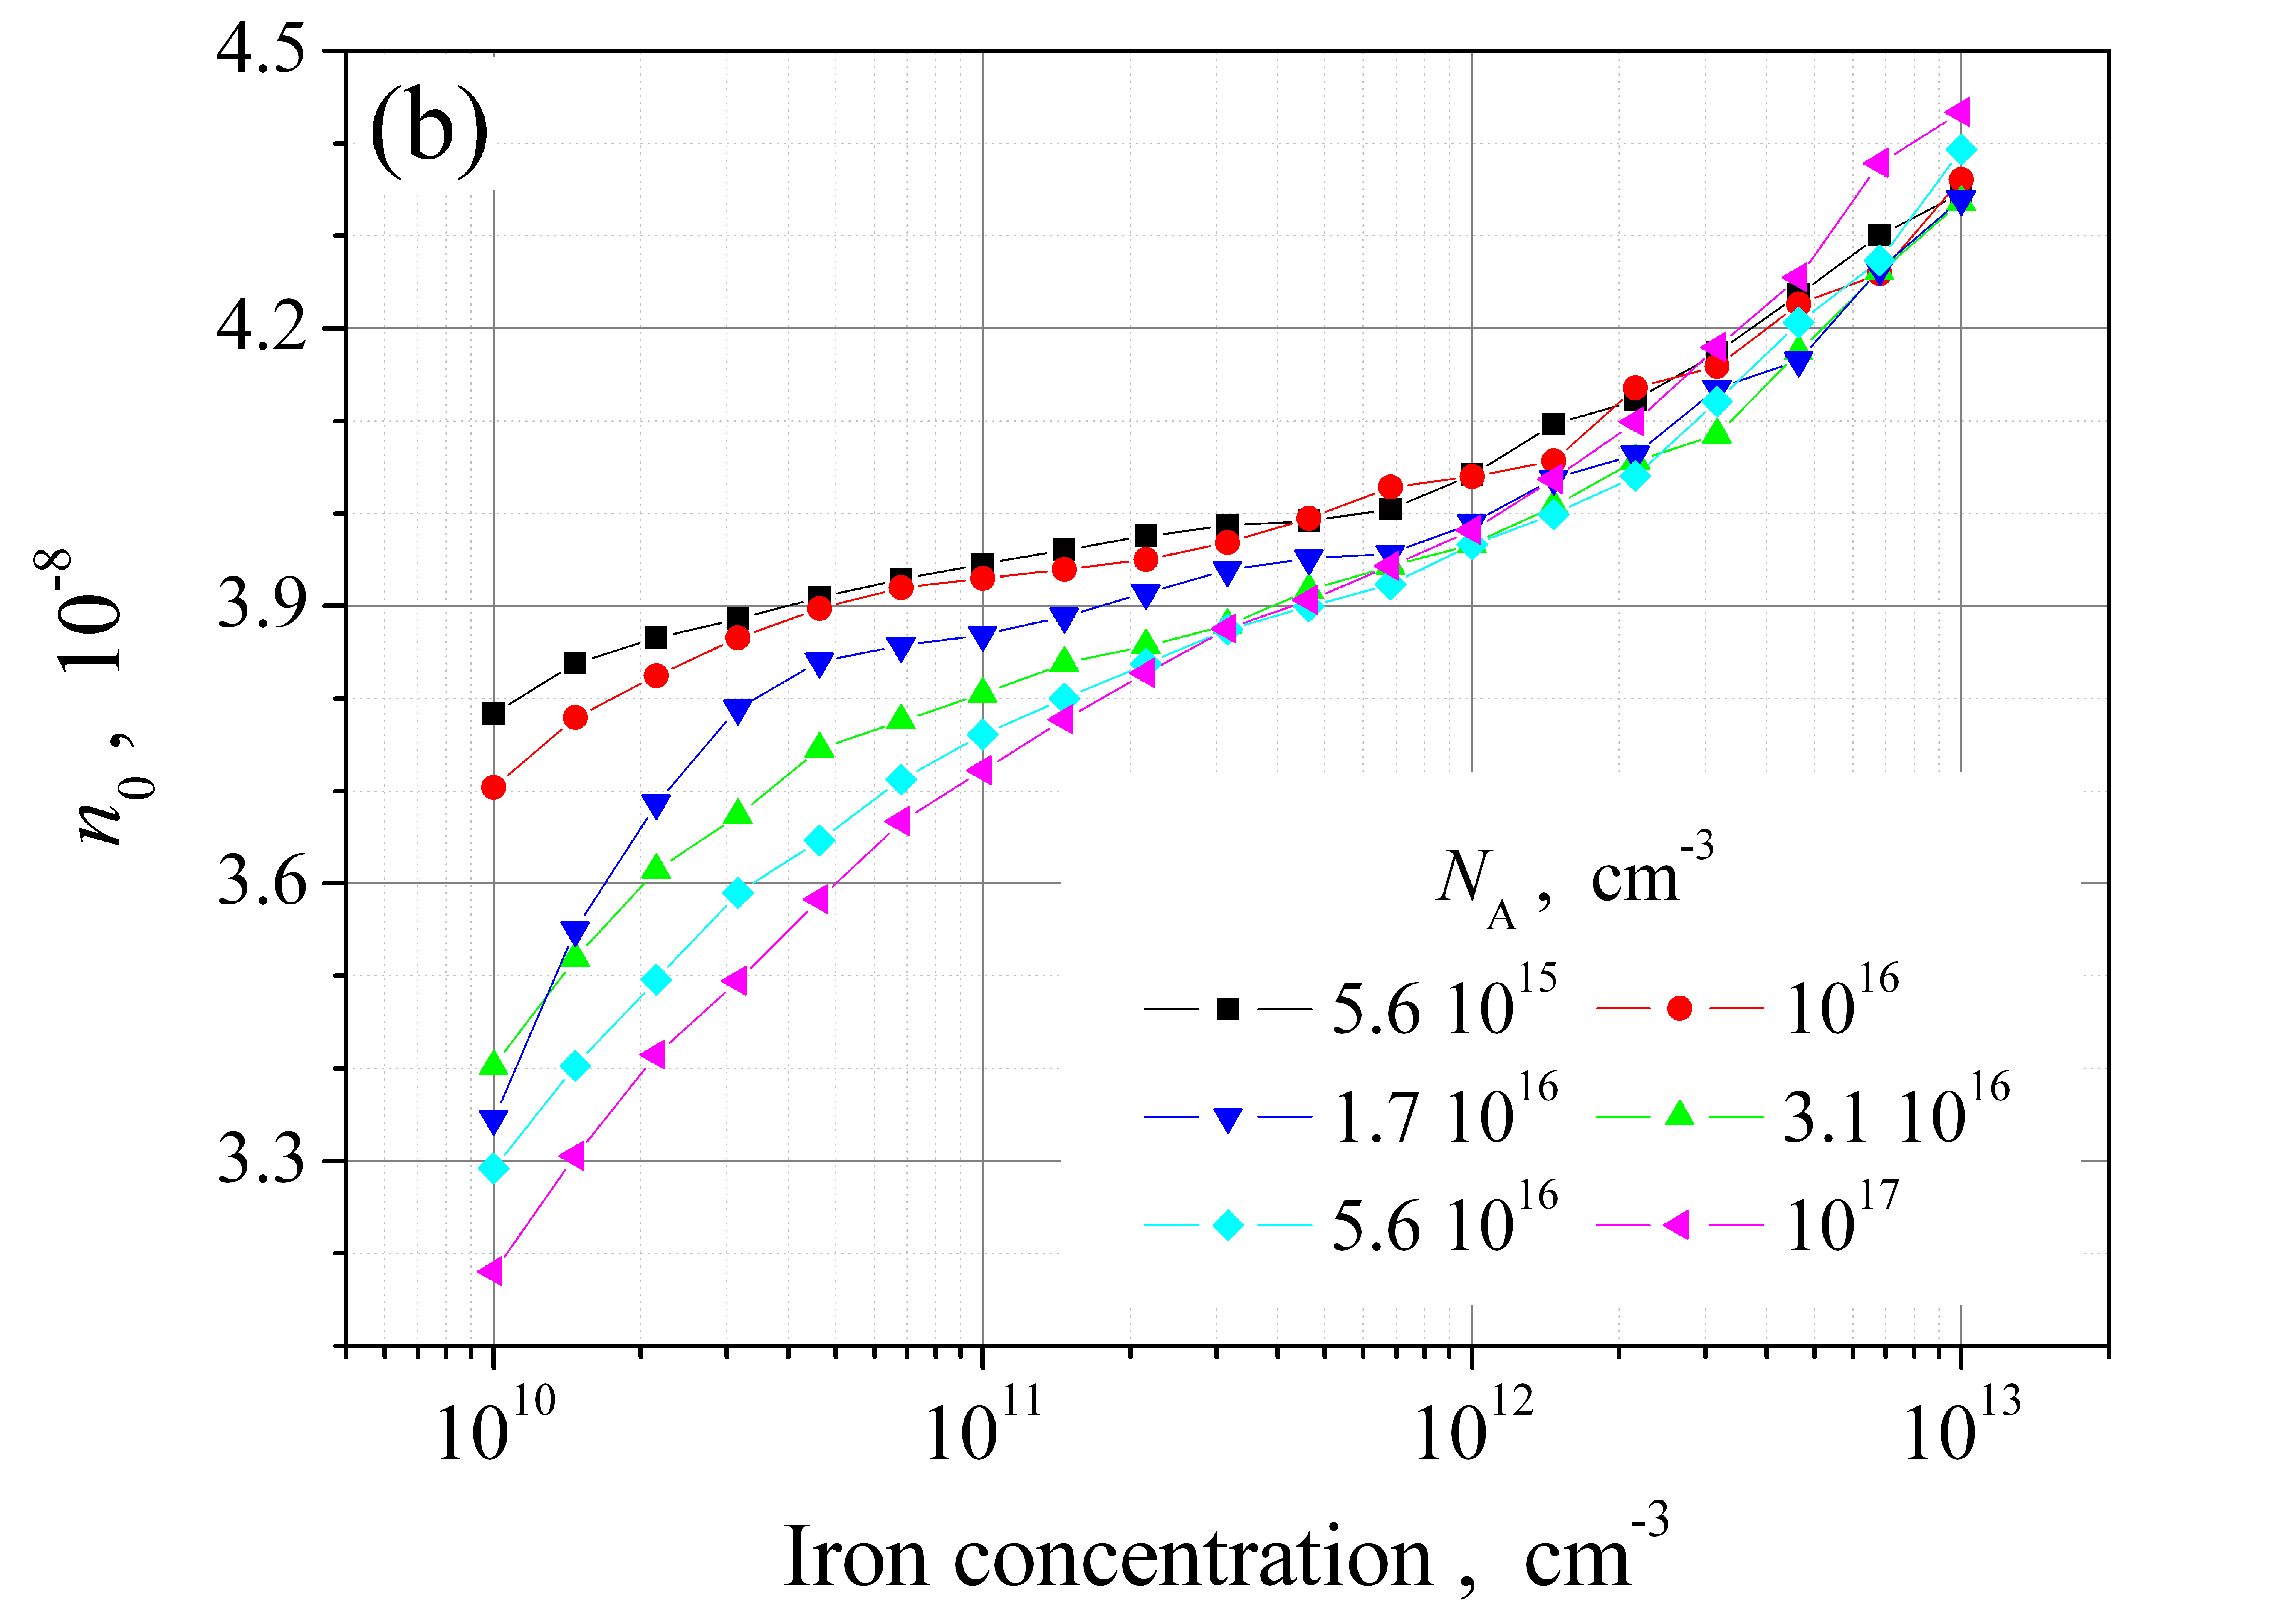
\includegraphics[width=0.5\textwidth]{Fig7b}
\caption{\label{fig7}
Dependencies of the parameters $\gamma$ (a) and $n_0$ (b) on the iron concentration in SC base.
FI--SRHBBA  case.
Lines in panel (a) are the fitted curves using Eq.~(\ref{eqGamma}), lines in panel (b) only
serve as guide to the eye.
}%
\end{figure}

\subsection{Fe--B pair and interstitial iron}


\begin{figure}
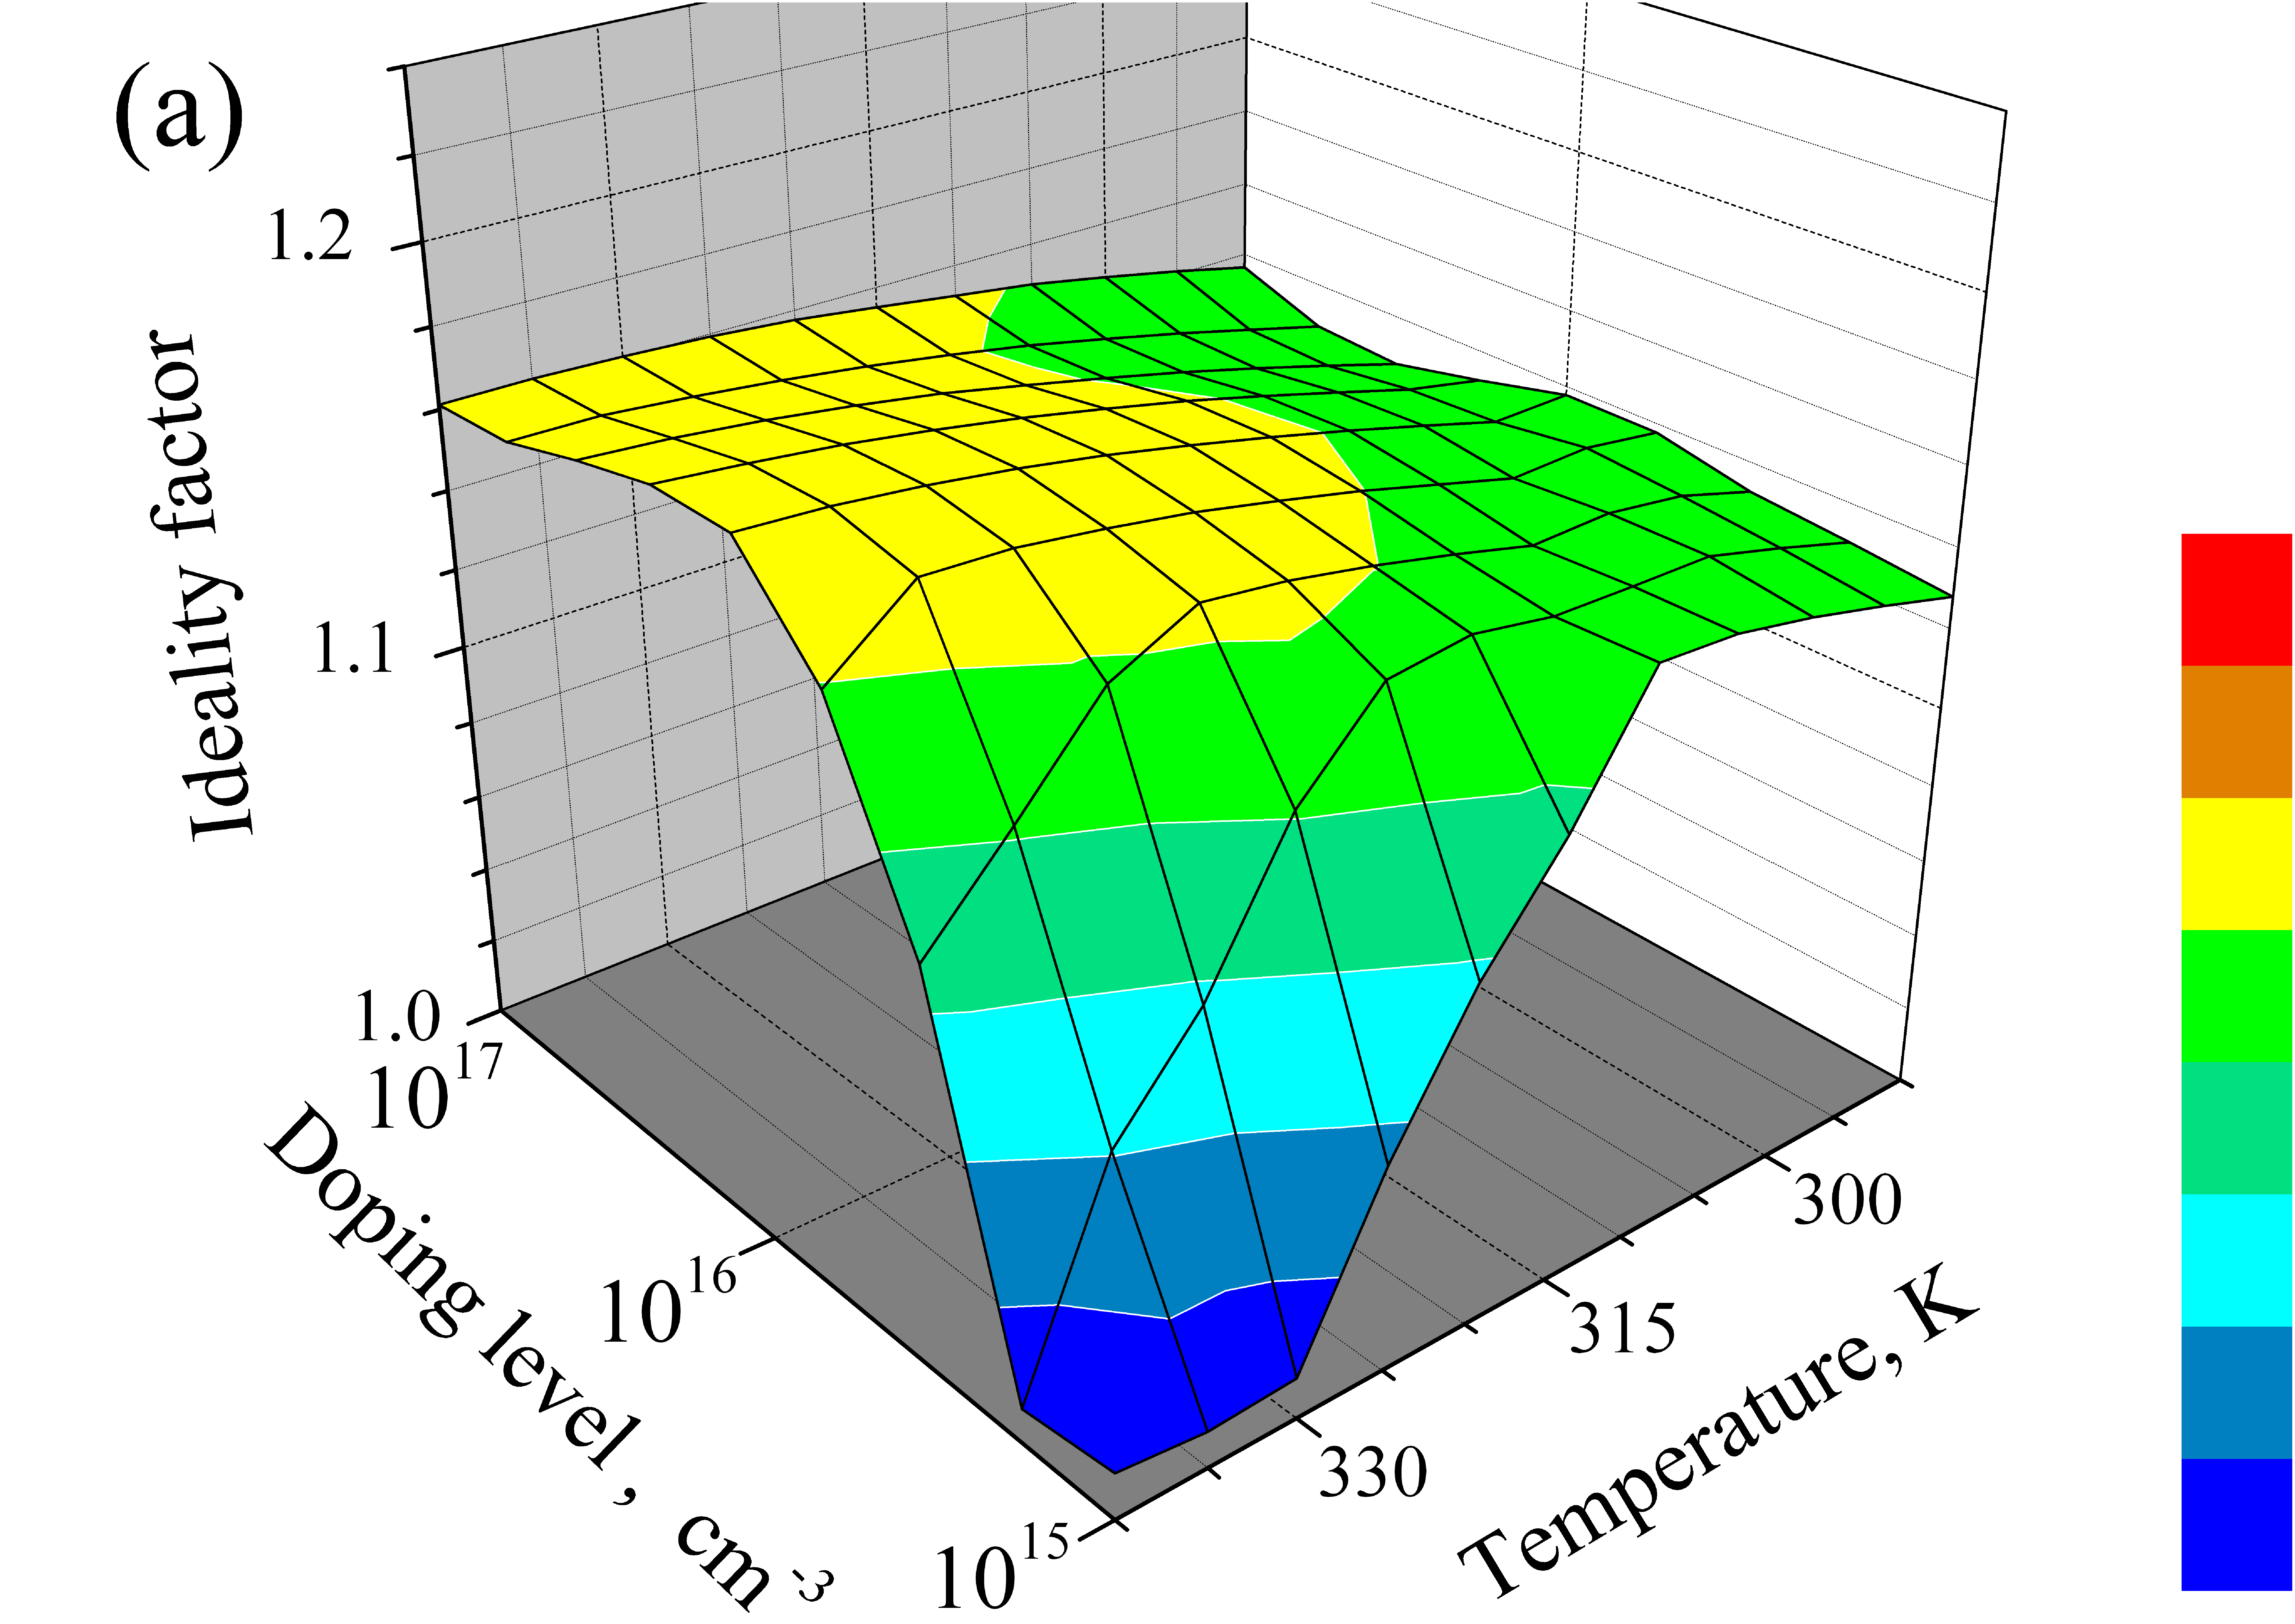
\includegraphics[width=0.5\textwidth]{Fig8a}%
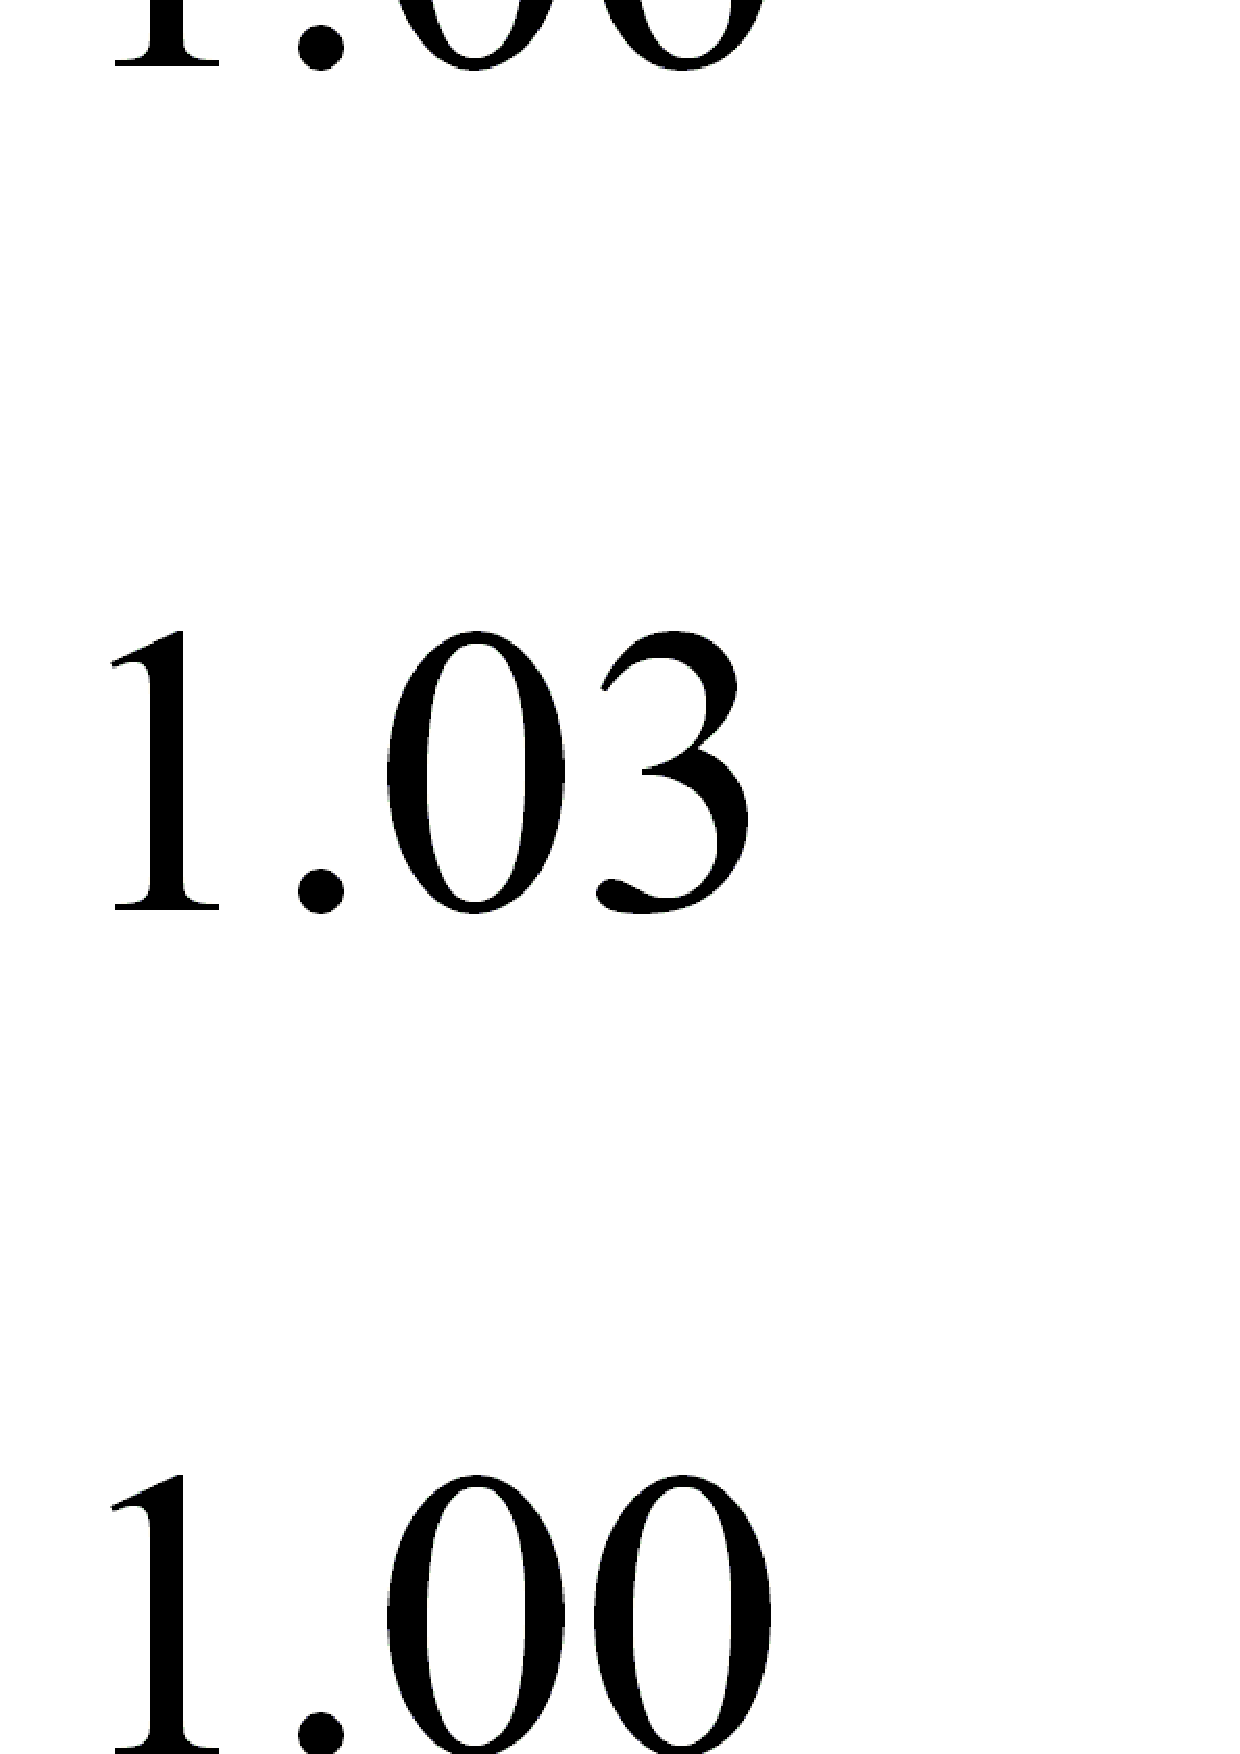
\includegraphics[width=0.5\textwidth]{Fig8b}

\includegraphics[width=0.5\textwidth]{Fig8c}
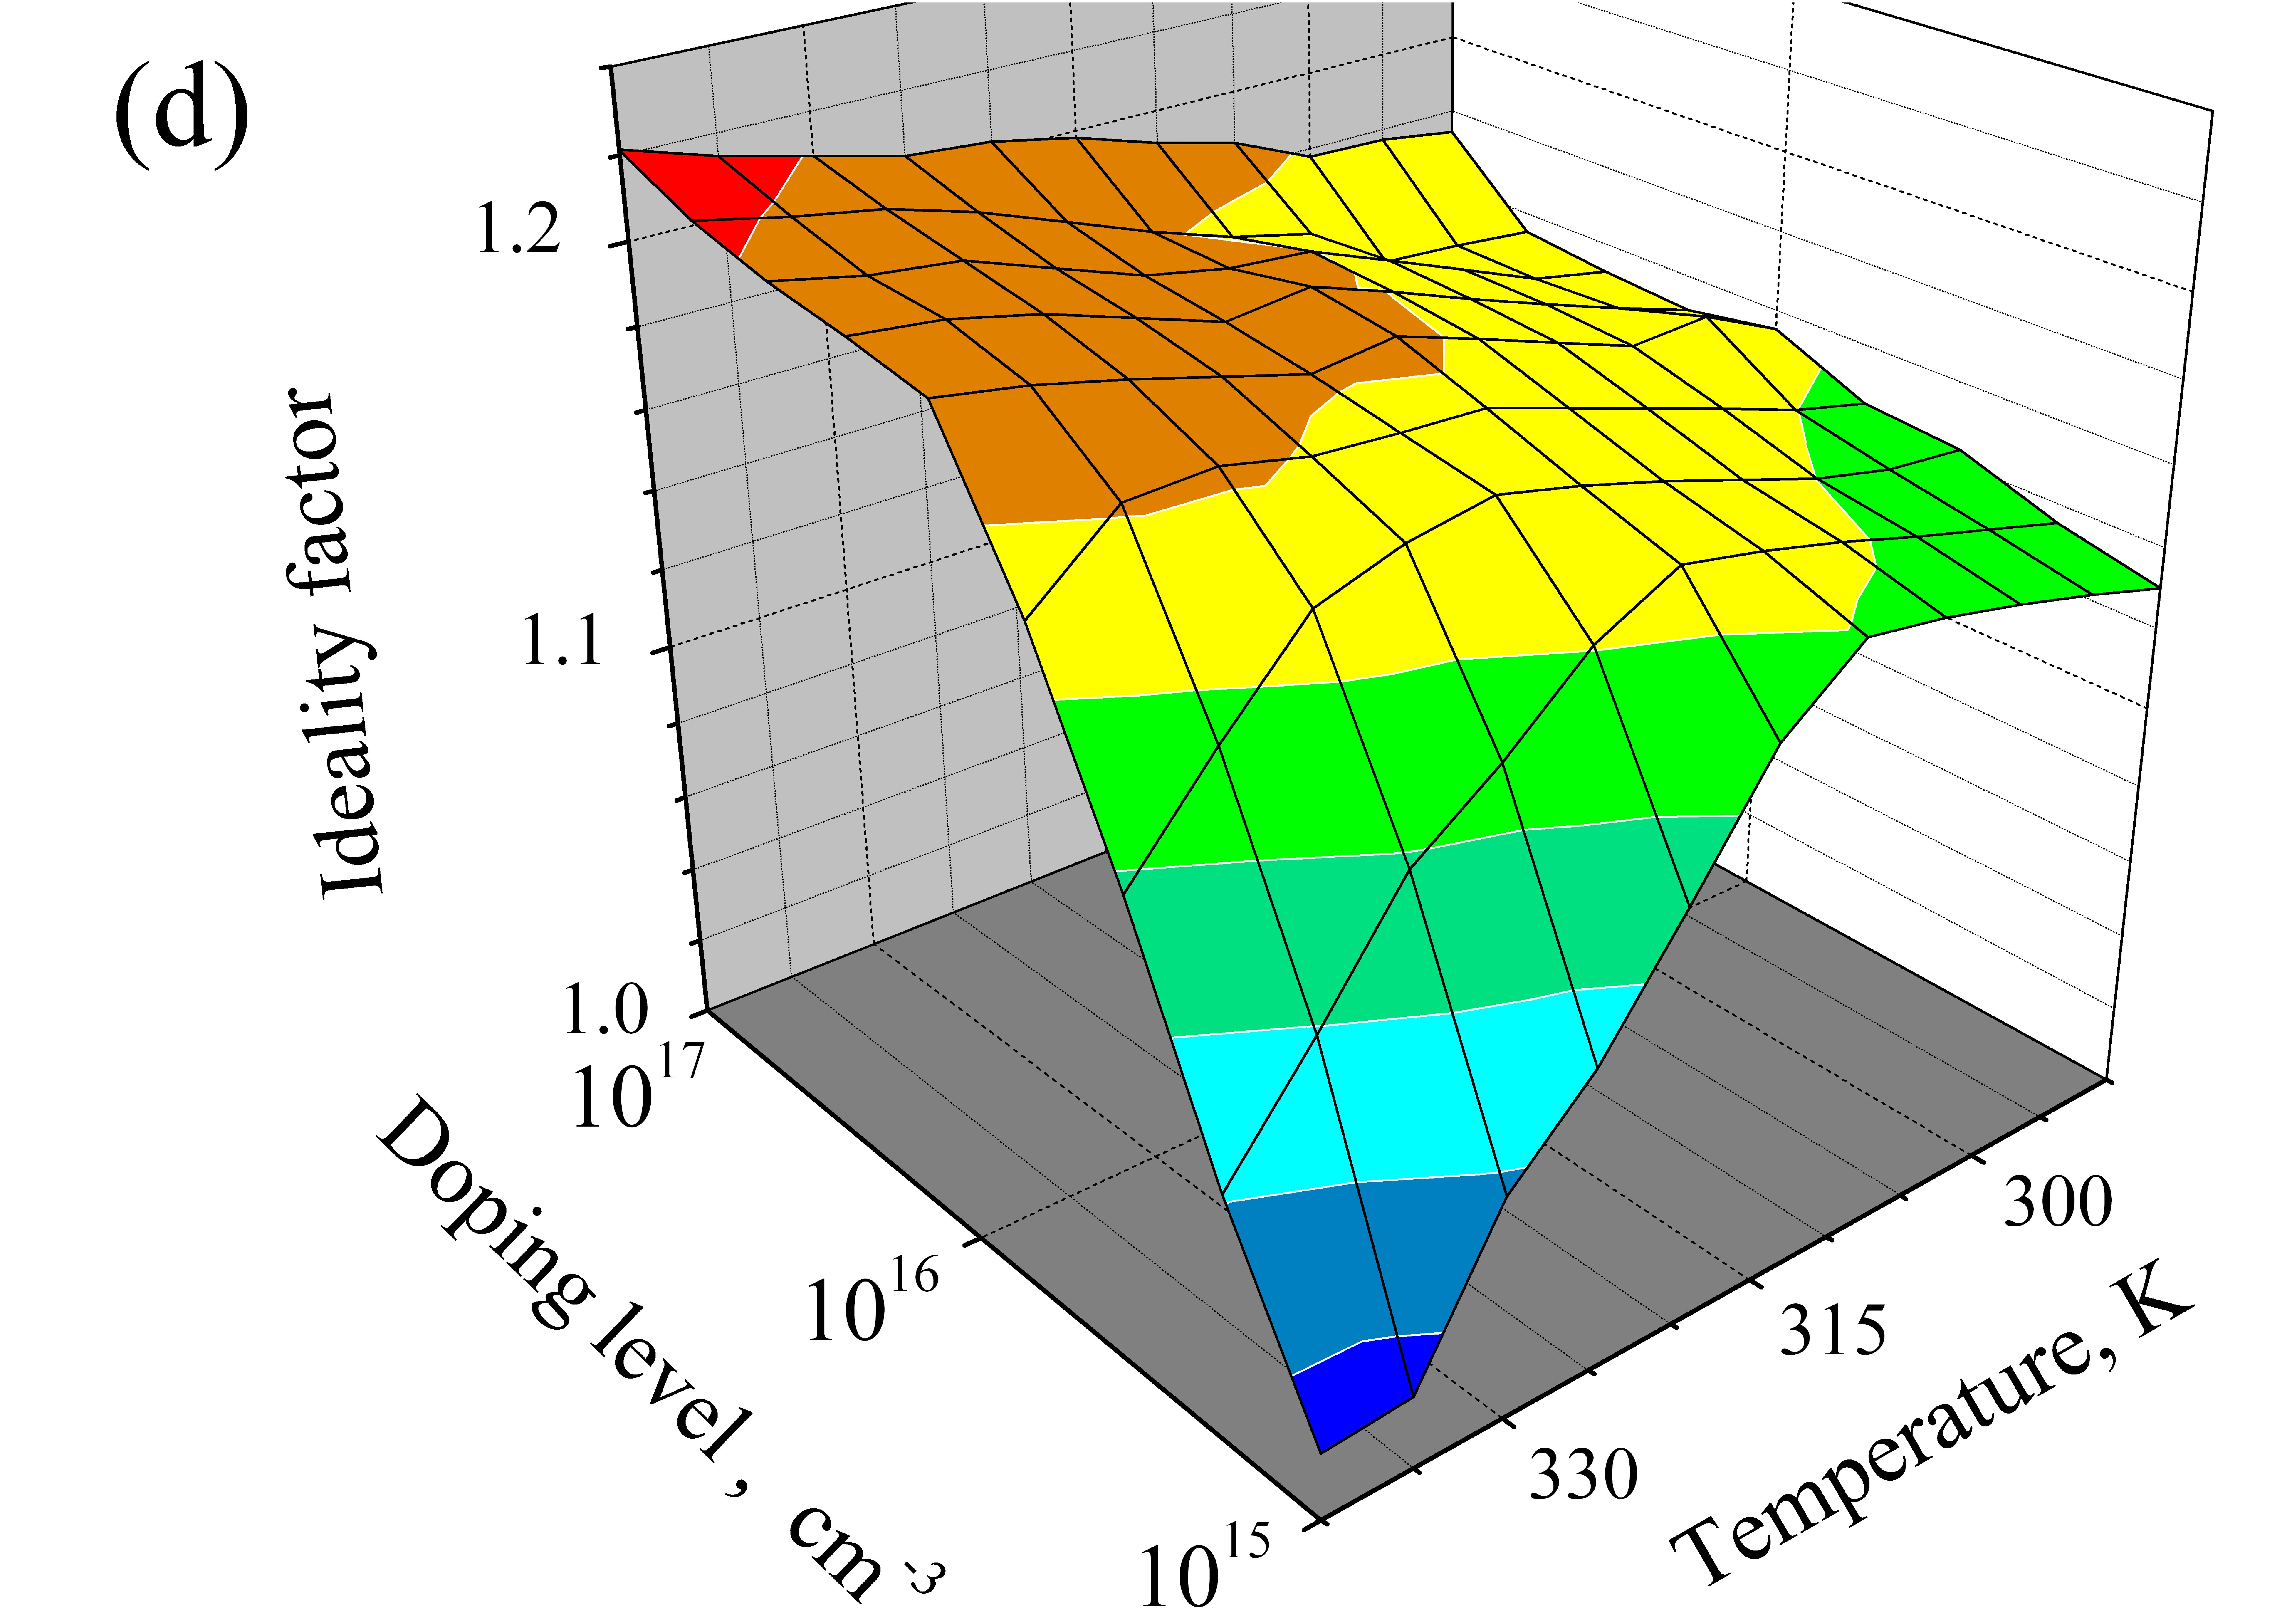
\includegraphics[width=0.5\textwidth]{Fig8d}
\caption{\label{fig8}
Ideality factor as a function of the temperature and dopant (boron) concentration.
FIFB--SRH (a,b) and FIFB--SRHBBA (c, d) cases.
$N_\mathrm{Fe}$, cm$^{-3}$: $10^{10}$ (a,c), $10^{13}$ (b,d).
}%
\end{figure}


\begin{figure}
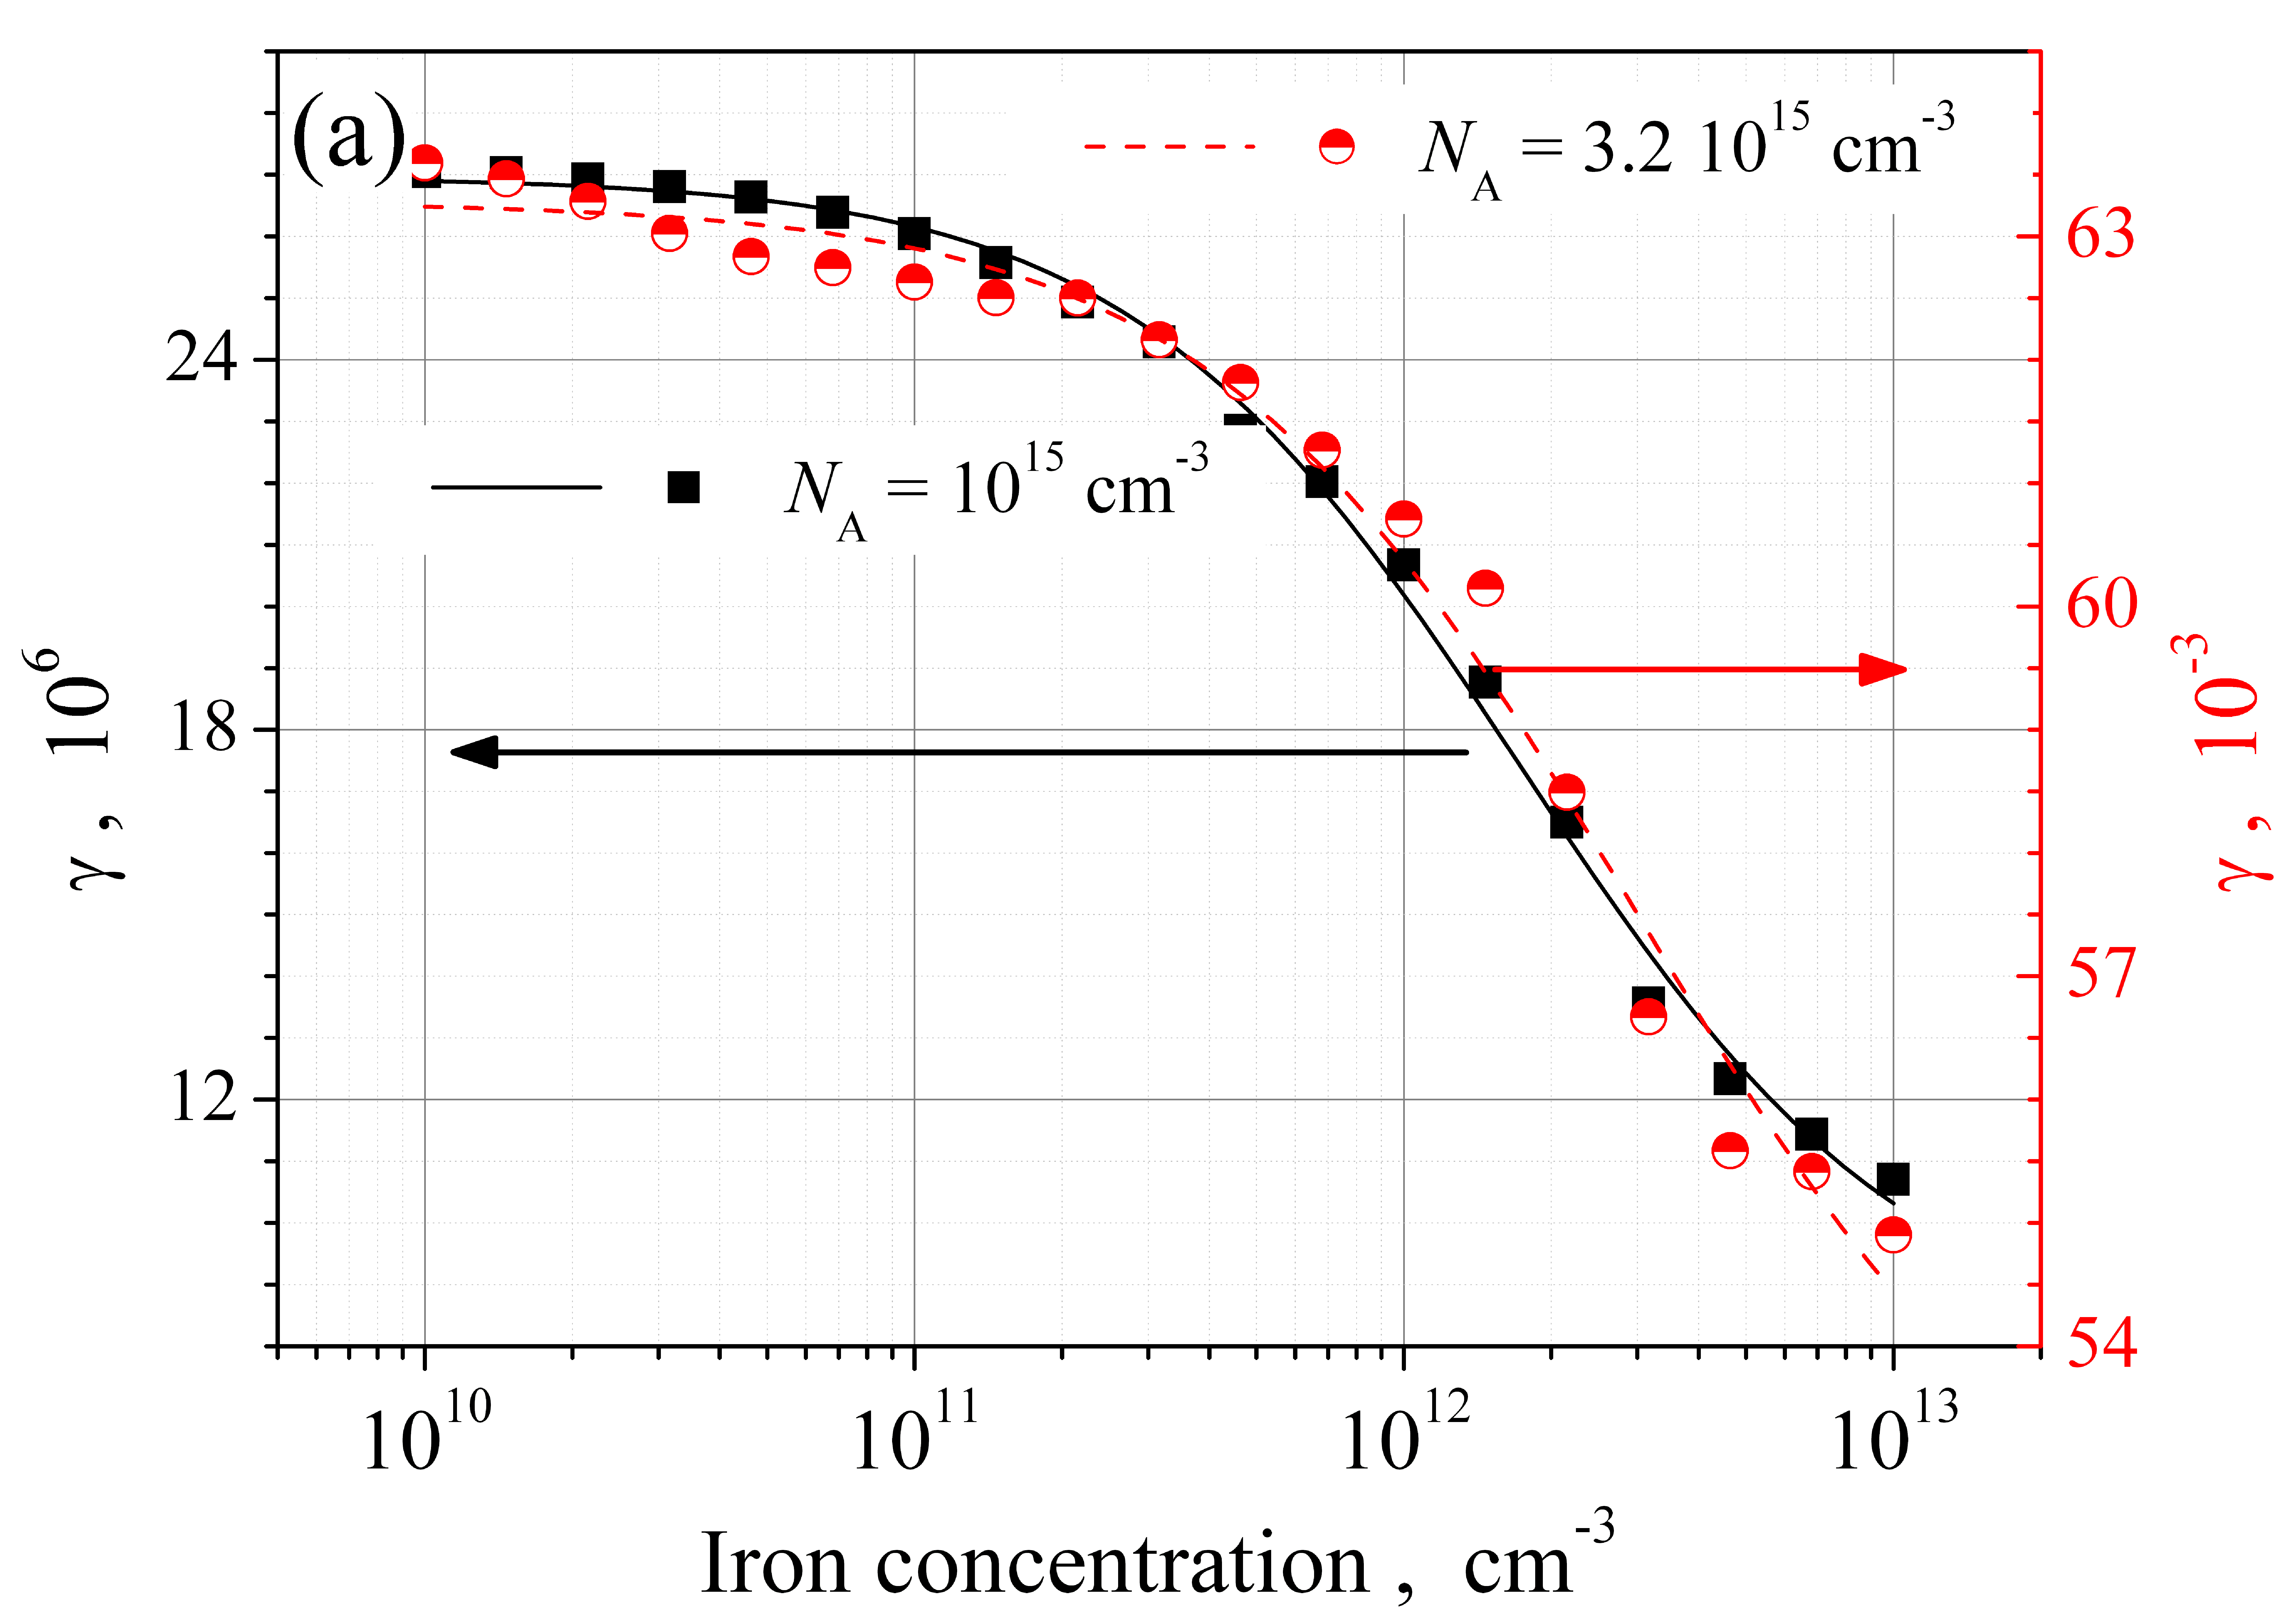
\includegraphics[width=0.5\textwidth]{Fig9a}%

\includegraphics[width=0.5\textwidth]{Fig9b}
\caption{\label{fig9}
Dependencies of the parameters $\gamma$ on the iron concentration in SC base.
FIFB--SRH (a) and FIFB--SRHBBA (b) cases.
Lines are the fitted curves using Eq.~(\ref{eqGamma})
}%
\end{figure}

\begin{figure}
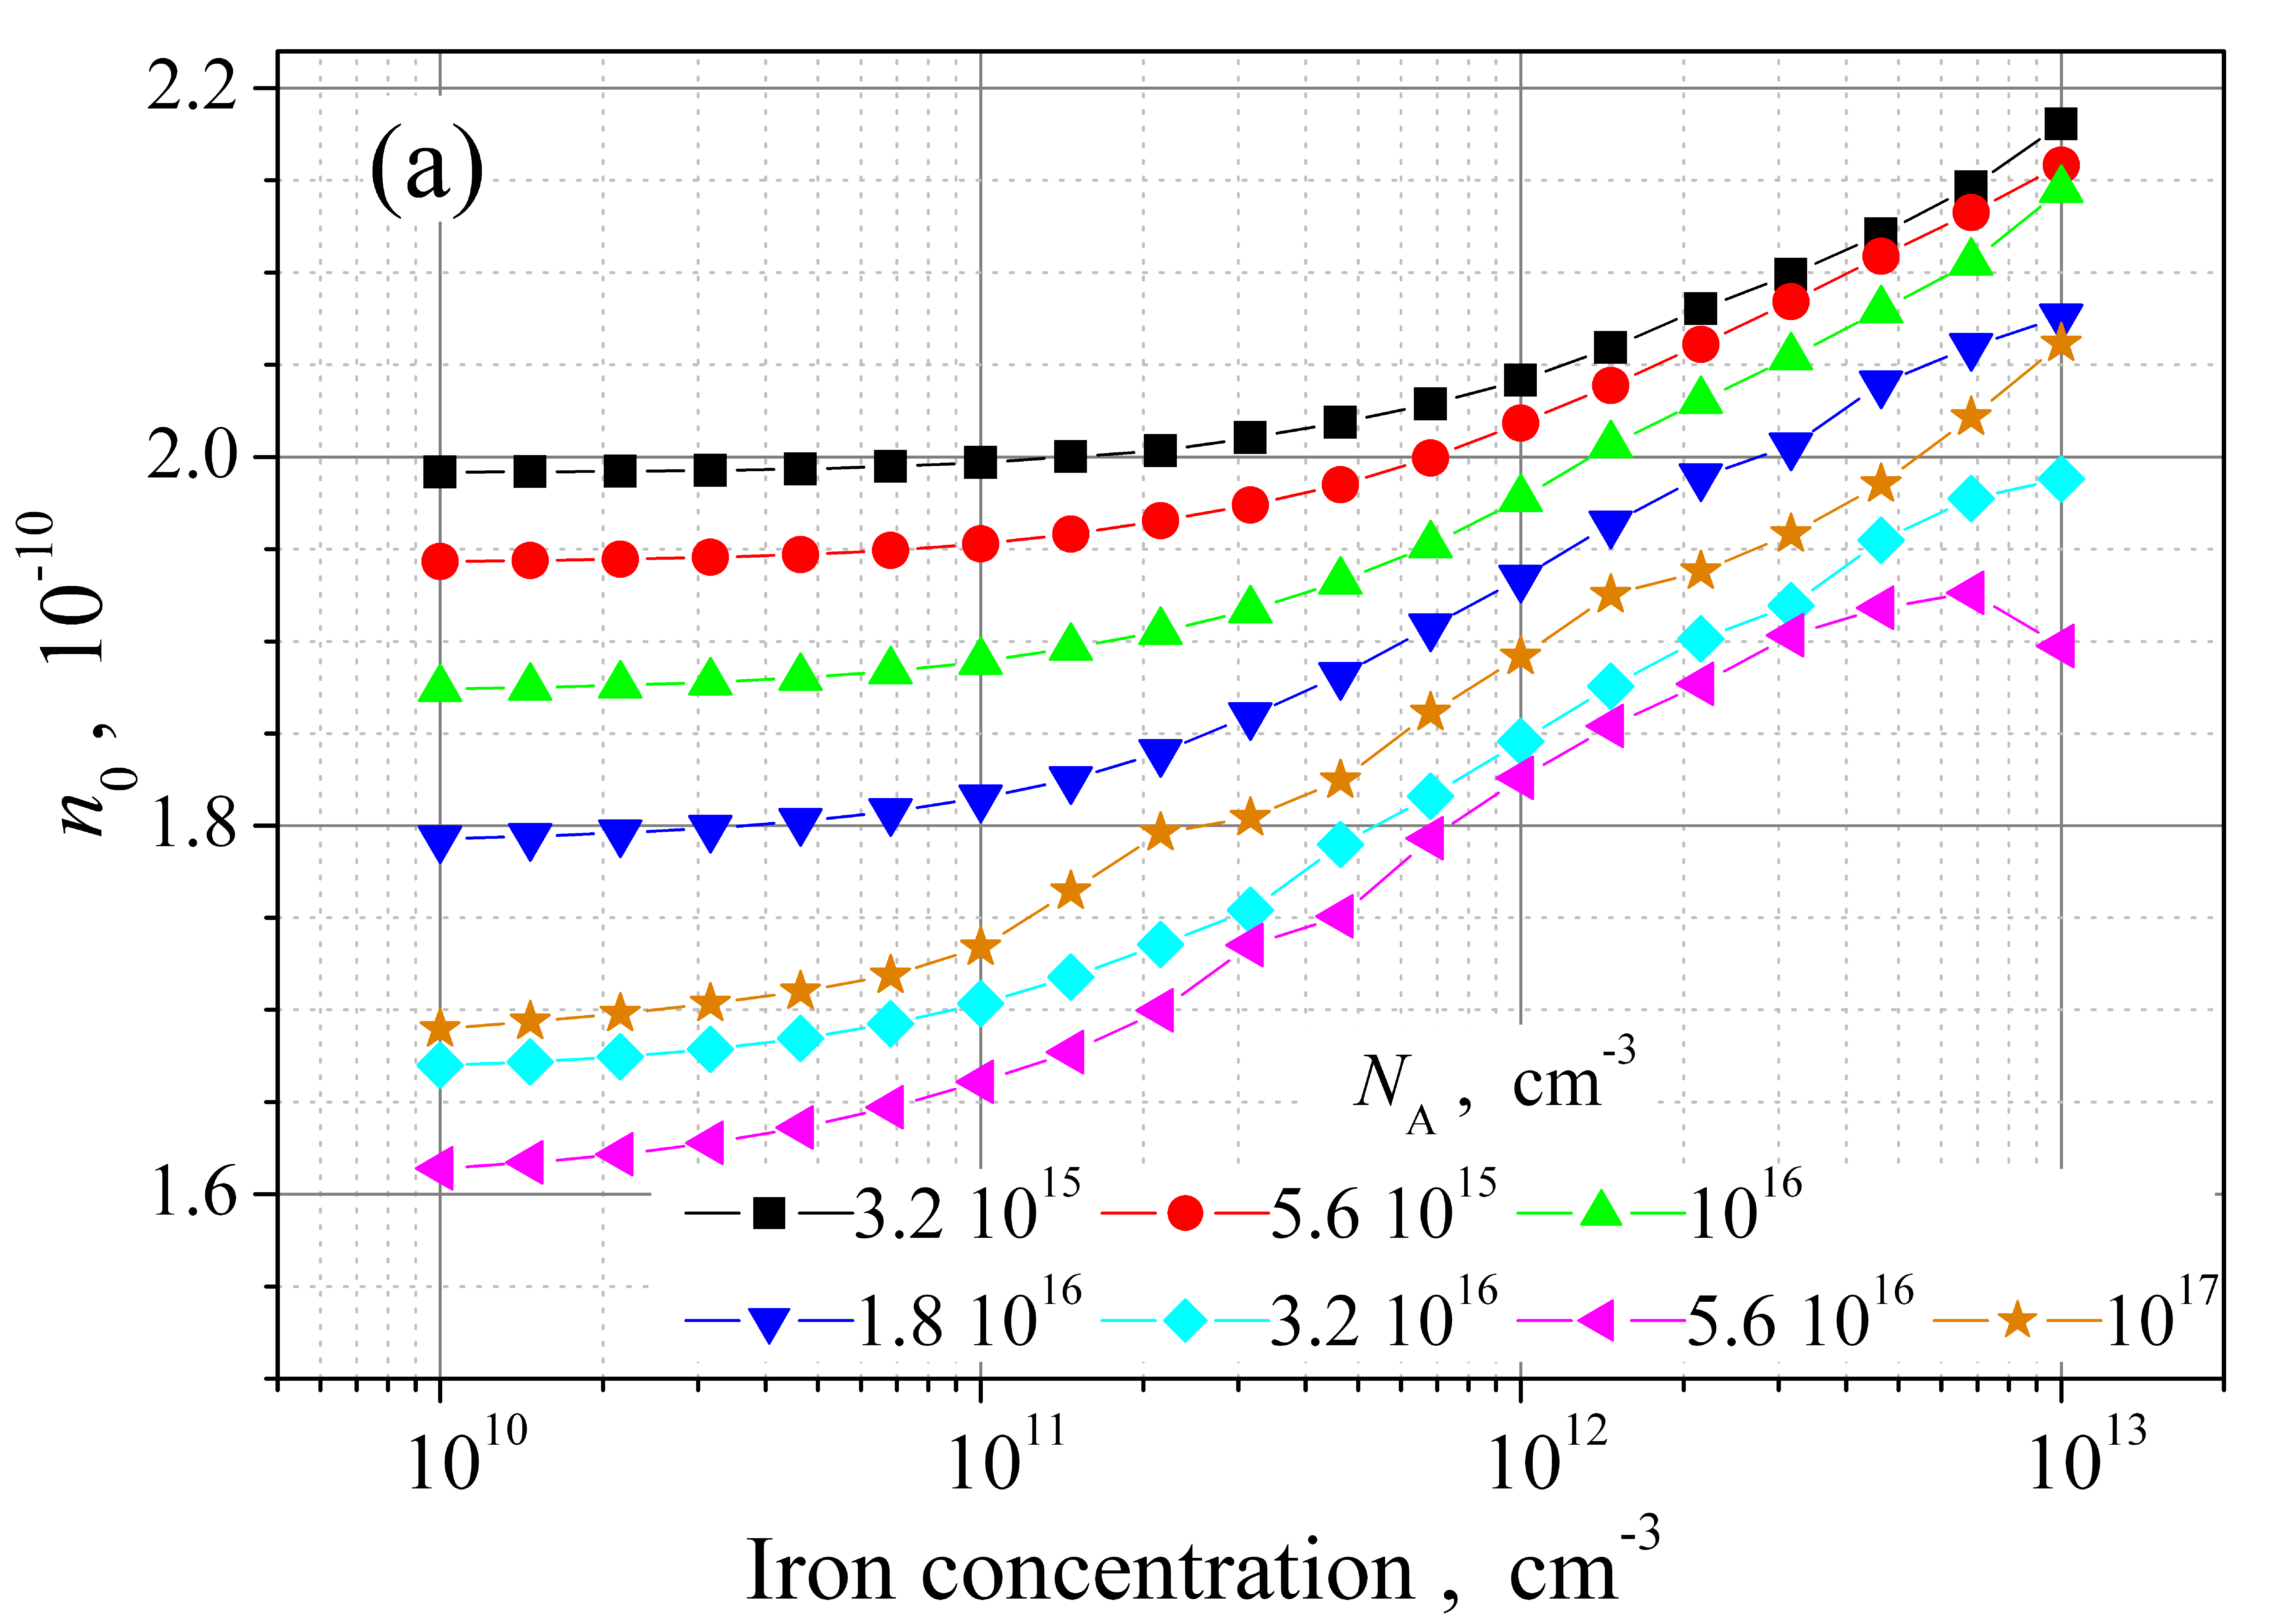
\includegraphics[width=0.5\textwidth]{Fig10a}%
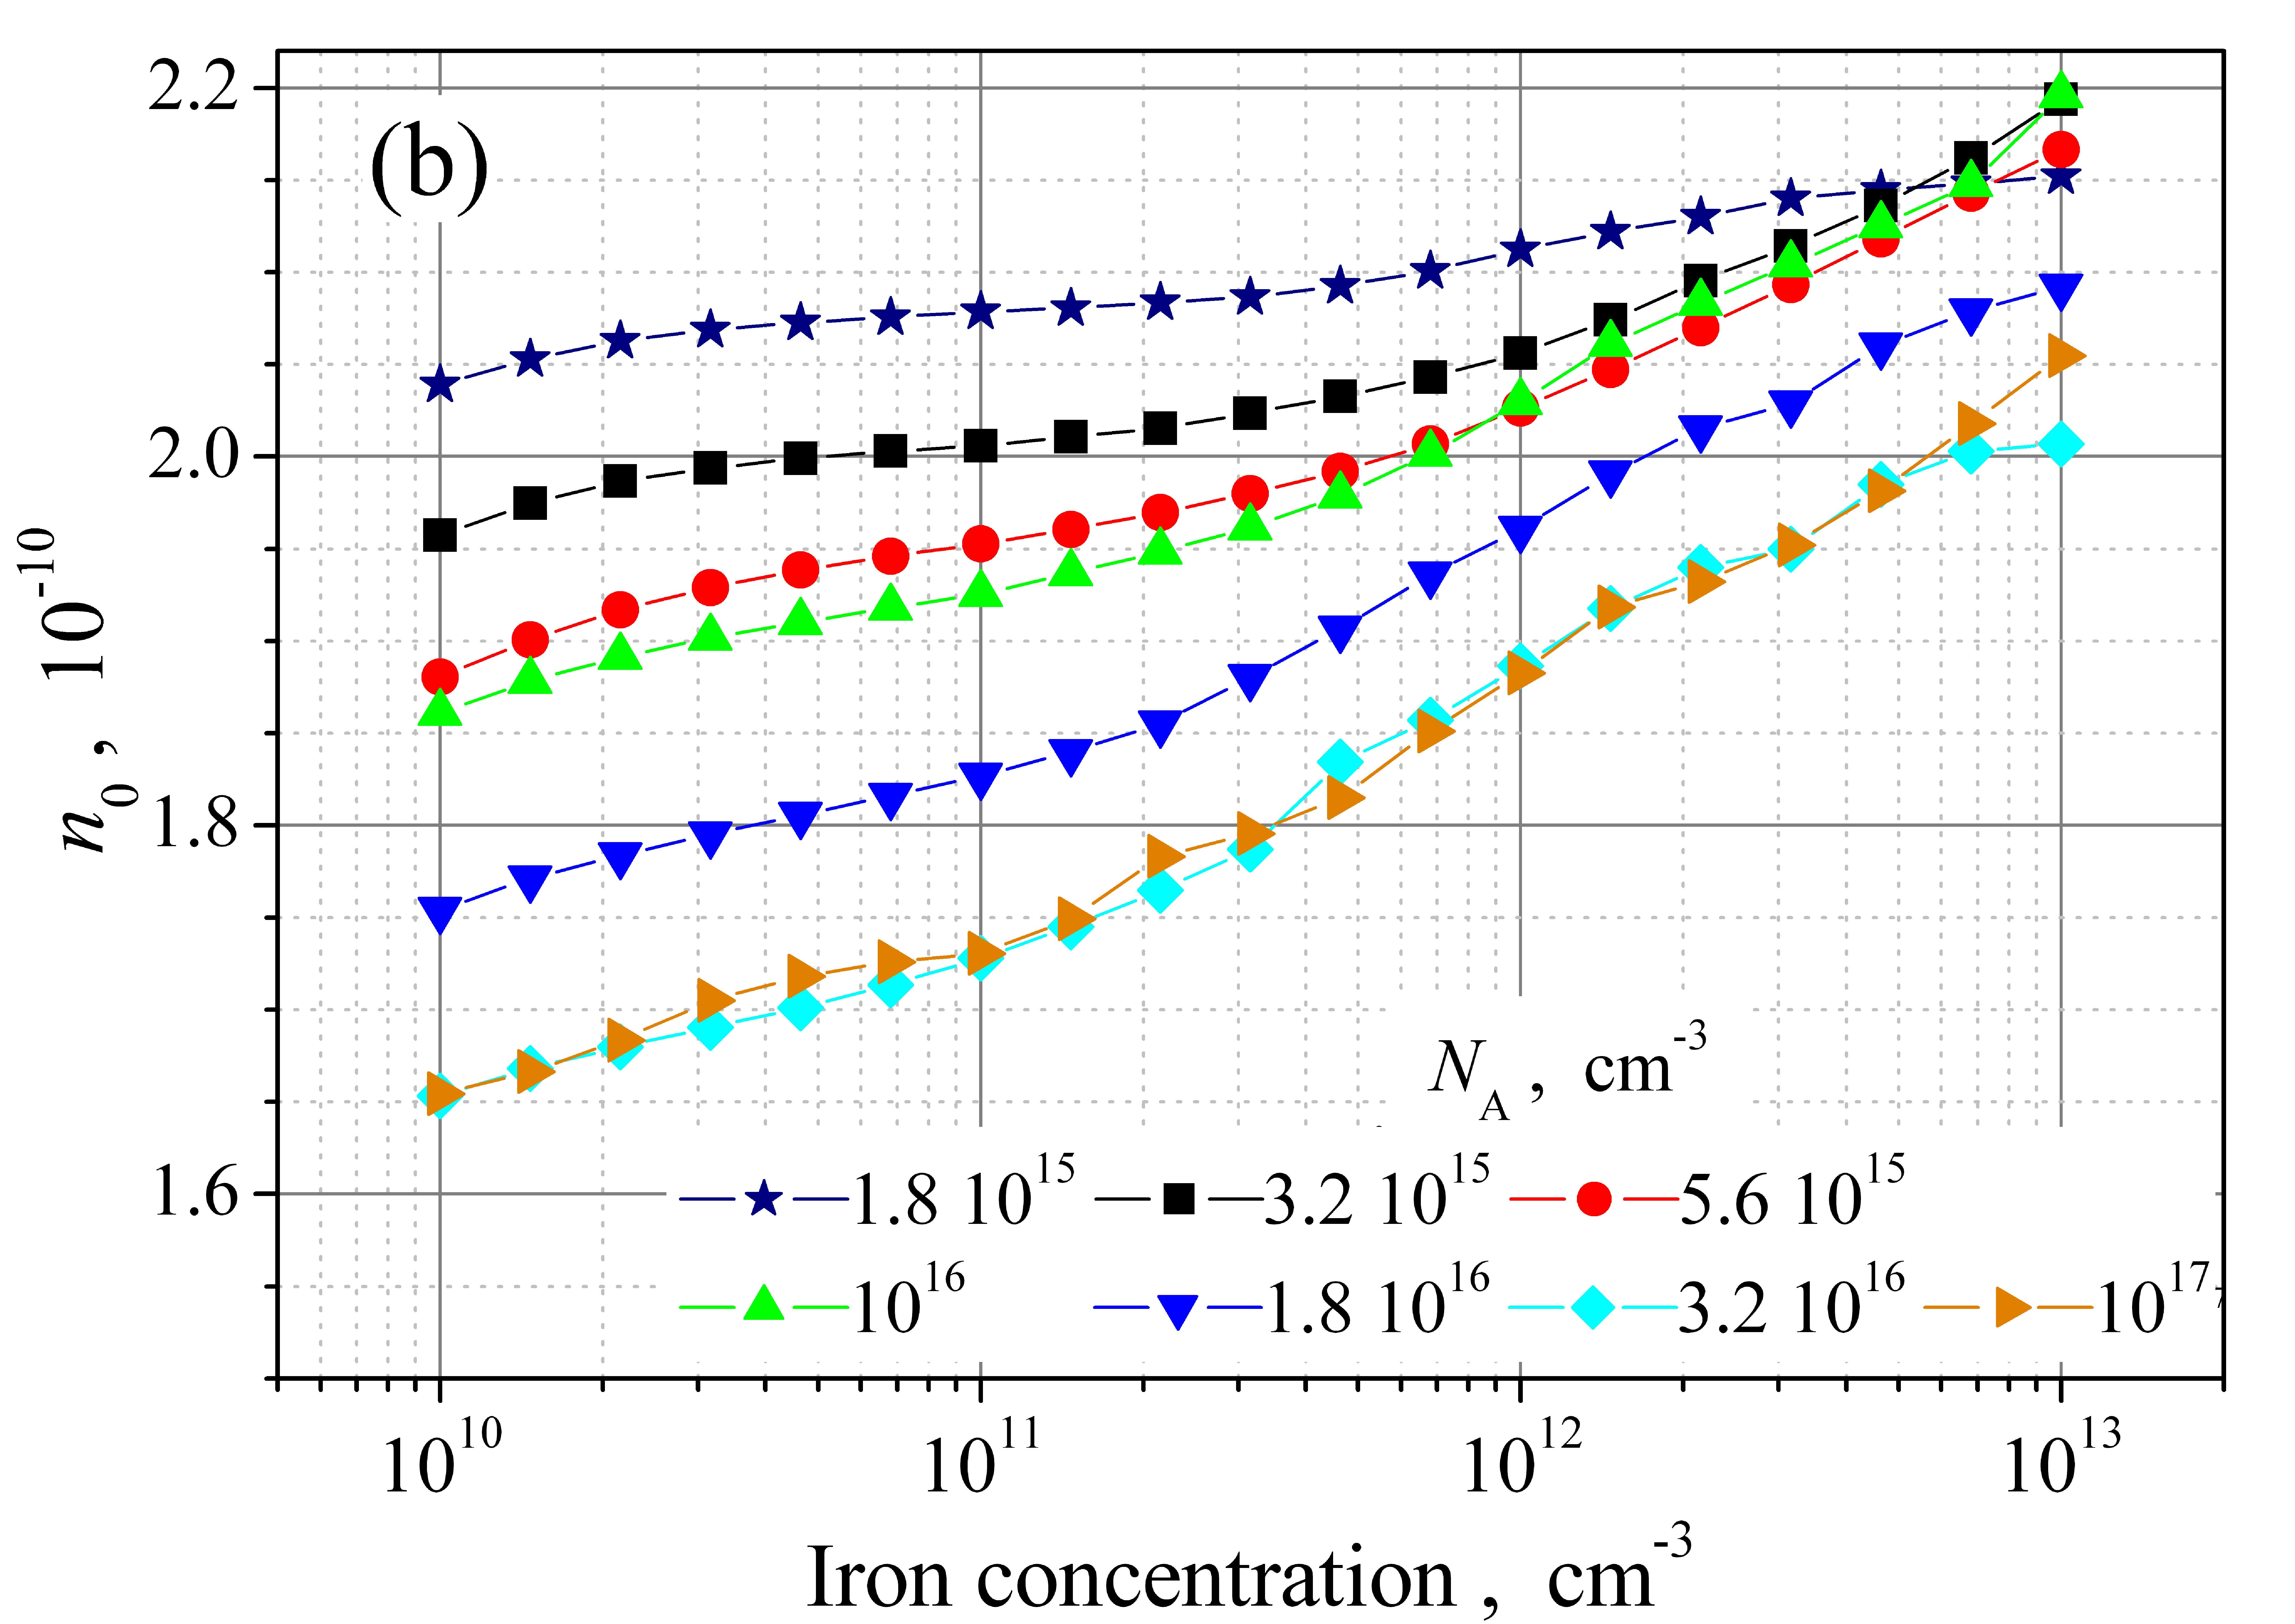
\includegraphics[width=0.5\textwidth]{Fig10b}
\caption{\label{fig10}
Dependencies of the parameters $n_0$ on the iron concentration in SC base.
FIFB--SRH (a) and FIFB--SRHBBA (b) cases.
Lines only serve as guide to the eye.
}%
\end{figure}




\section{Conclusion and further plan}
The influence of ultrasound on the silicon solar cell  has been investigated experimentally over a temperature range of 290--340~K.
The investigation has revealed an acoustically driven reversible degradation in SSC parameters.
The effect is intensified in the case of the transverse acoustic waves using.
The analysis has shown that degradation is caused by the acoustically induced increase in the carrier capture coefficient for point or extended defects.
The qualitative model of the observed phenomenon, which is based on the increase in the distance between coupled defects or between complex defect components due to ultrasound action, has been considered.
It has been shown that the oxide precipitates are most likely defects, which take part in the acousto--defect interaction.
Thus, ultrasound can be an effective tool for controlling silicon structure characteristics.



\section*{References}

\bibliography{olikh}


\end{document}

